% % !TeX root = tcolorbox.tex
% % include file of tcolorbox.tex (manual of the LaTeX package tcolorbox)
% %\clearpage
\section{Library \mylib{skins}}\label{sec:skins}%
\tcbset{external/prefix=external/skins_}%
The library is loaded by a package option or inside the preamble by:

可以通过包选项或在导言区内加载以下命令来加载该库
\begin{dispListing}
\tcbuselibrary{skins}
\end{dispListing}
This also loads the package |tikz| \cite{tantau:tikz_and_pgf}. Typically but not necessarily,
the following skins use |tikz| instead of |pgf|.

这也会加载|tikz|包\cite{tantau:tikz_and_pgf}。通常情况下,但并不一定,下面的皮肤会使用|tikz|而不是|pgf|。

In the following, general settings and options of the library are
documented.
The actual catalog of skins is found in \Vref{sec:skincatalog}.

以下记录了该库的一般设置和选项。皮肤目录实际上在\Vref{sec:skincatalog}中。

% \subsection{Style Option Keys\\样式选项键}\label{subsec:addstyleoptions}
% The following style options are applicable for all skins which
use engines of type |path|, |pathfirst|, |pathmiddle|, or |pathlast|.
Especially, the skin \refSkin{enhanced} supports \emph{all} of them
and \refSkin{standard} \emph{none}.

以下样式选项适用于所有使用类型为 |path|、|pathfirst|、|pathmiddle| 或 |pathlast| 的引擎的皮肤。特别地,皮肤 \refSkin{enhanced} 支持 \emph{所有} 这些选项,而皮肤 \refSkin{standard} 则不支持任何一个。


\begin{docTcbKey}{frame style}{=\meta{\texttt{\upshape tikz} keys}}{style, no default}
The \meta{\texttt{\upshape tikz} keys} are used inside the |tikz| path command
for drawing the \emph{frame} of the box.\\
This option is available if the \refKey{/tcb/frame engine} is set to
|path|, |pathfirst|, |pathmiddle|, or |pathlast|.
It is \emph{not} available for |standard|.

\meta{\texttt{\upshape tikz} keys}被用于在|tikz|路径命令中绘制盒子的\emph{框架}。\ 如果\refKey{/tcb/frame engine}设置为|path|、|pathfirst|、|pathmiddle|或|pathlast|,则此选项可用。对于|standard|,它是\emph{不可用}的。
\begin{exdispExample*}{frame_style}{sbs,lefthand ratio=0.66}
\tcbset{colback=red!5!white,fonttitle=\bfseries}

\begin{tcolorbox}[enhanced,title=My title,
frame style={left color=red!75!black,
              right color=blue!75!black}]
This is a \textbf{tcolorbox}.
\tcblower
This is the lower part.
\end{tcolorbox}
\end{exdispExample*}
\end{docTcbKey}

\begin{docTcbKey}{frame style image}{=\meta{file name}}{no default, initially unset}
Fills the frame with an external image referenced by \meta{file name}.
For advanced features like blending of a picture with the background,
use \refKey{/tcb/frame style} together with \refKey{/tikz/fill stretch image}.

使用 \meta{文件名} 引用外部图像来填充帧。要使用高级功能,例如将图像与背景混合,可以同时使用 \refKey{/tcb/frame style} 和 \refKey{/tikz/fill stretch image}。
\begin{exdispExample*}{frame_style_image}{sbs,lefthand ratio=0.66}
\tcbset{colback=red!5!white,fonttitle=\bfseries}

\begin{tcolorbox}[enhanced,title=My title,
  frame style image=blueshade.png]
This is a \textbf{tcolorbox}.
\tcblower
This is the lower part.
\end{tcolorbox}
\end{exdispExample*}
\end{docTcbKey}

% %\clearpage
\begin{docTcbKey}{frame style tile}{=\marg{graphics options}\marg{file name}}{no default, initially unset}
Fills the frame with a tile pattern based on an external image referenced by \meta{file name}.
The \meta{graphics options} are given to the underlying \docAuxCommand*{includegraphics} command.
For advanced features like blending of a picture with the background,
use \refKey{/tcb/frame style} together with \refKey{/tikz/fill tile image}.

根据外部引用的文件名为\meta{file name}的图像,填充框架以形成平铺图案。 \meta{graphics options}提供给底层的\docAuxCommand*{includegraphics}命令。对于高级功能,如将图片与背景混合,可使用\refKey{/tcb/frame style}和\refKey{/tikz/fill tile image}。
\begin{exdispExample*}{frame_style_tile}{sbs,lefthand ratio=0.66}
\tcbset{colback=red!5!white,coltitle=red!30!black,
  opacityback=0.75,fonttitle=\bfseries}

\begin{tcolorbox}[enhanced,title=My title,
  frame style tile={width=1cm}{pink_marble.png}]
This is a \textbf{tcolorbox}.
\tcblower
This is the lower part.
\end{tcolorbox}
\end{exdispExample*}
\end{docTcbKey}

\begin{docTcbKey}{frame hidden}{}{style, no value}
This is a shortcut for |frame style={draw=none,fill=none}|.
Depending on the skin, this option switches off the drawing of the
frame.
Alternatively, use \refKey{/tcb/frame empty}.

这是一个快捷方式,用于设置 |frame style={draw=none,fill=none}|。 根据皮肤不同,此选项可以关闭框架的绘制。 或者,可以使用 \refKey{/tcb/frame empty}。
\begin{exdispExample*}{frame_hidden}{sbs,lefthand ratio=0.66}
\tcbset{colback=red!5!white,colframe=red!75!black,
fonttitle=\bfseries,coltitle=black}

\begin{tcolorbox}[enhanced,title=My title,
frame hidden]
This is a \textbf{tcolorbox}.
\tcblower
This is the lower part.
\end{tcolorbox}
\end{exdispExample*}
\end{docTcbKey}


\begin{docTcbKey}{interior style}{=\meta{\texttt{\upshape tikz} keys}}{style, no default}
The \meta{\texttt{\upshape tikz} keys} are used inside the |tikz| path command
for drawing the \emph{interior} of the box. They are used for the titled
and for the untitled version as well.\\
This option is available if the \refKey{/tcb/interior titled engine}
or \refKey{/tcb/interior engine} is set to
|path|, |pathfirst|, |pathmiddle|, or |pathlast|.
It is \emph{not} available for |standard|.

\meta{\texttt{\upshape tikz} keys} 用于在 |tikz| 路径命令中绘制盒子的\emph{内部}。无论是有标题还是无标题版本都会用到它们。\\ 如果设置了 \refKey{/tcb/interior titled engine} 或 \refKey{/tcb/interior engine} 为 |path|、|pathfirst|、|pathmiddle| 或 |pathlast|,则可使用此选项。但对于 |standard|,此选项\emph{不可用}。
\begin{exdispExample*}{interior_style}{sbs,lefthand ratio=0.66}
\tcbset{colframe=red!75!black,fonttitle=\bfseries}

\begin{tcolorbox}[enhanced,title=My title,
interior style={left color=red!20!white,
                right color=yellow!50!white}]
This is a \textbf{tcolorbox}.
\tcblower
This is the lower part.
\end{tcolorbox}
\end{exdispExample*}
\end{docTcbKey}

% %\clearpage
\begin{docTcbKey}{interior style image}{=\meta{file name}}{no default, initially unset}
Fills the interior with an external image referenced by \meta{file name}.
For advanced features like blending of a picture with the background,
use \refKey{/tcb/interior style} together with \refKey{/tikz/fill stretch image}.

使用 \meta{文件名} 引用外部图像来填充内部。 对于像将图片与背景混合的高级功能, 请使用 \refKey{/tcb/interior style} 与 \refKey{/tikz/fill stretch image}。
\begin{exdispExample*}{interior_style_image}{sbs,lefthand ratio=0.66}
\tcbset{colframe=red!75!black,fonttitle=\bfseries}

\begin{tcolorbox}[enhanced,title=My title,
interior style image=goldshade.png]
This is a \textbf{tcolorbox}.
\tcblower
This is the lower part.
\end{tcolorbox}
\end{exdispExample*}
\end{docTcbKey}


\begin{docTcbKey}{interior style tile}{=\marg{graphics options}\marg{file name}}{no default, initially unset}
Fills the interior with a tile pattern based on an external image referenced by \meta{file name}.
The \meta{graphics options} are given to the underlying \docAuxCommand*{includegraphics} command.
For advanced features like blending of a picture with the background,
use \refKey{/tcb/interior style} together with \refKey{/tikz/fill tile image}.

根据外部的图像文件名\meta{file name},填充内部具有瓷砖图案。 \meta{graphics options}将传递给底层的\docAuxCommand*{includegraphics}命令。对于高级功能,例如将图片与背景混合,可以使用\refKey{/tcb/interior style}和\refKey{/tikz/fill tile image}。
\begin{exdispExample*}{interior_style_tile}{sbs,lefthand ratio=0.66}
\tcbset{colframe=red!75!black,fonttitle=\bfseries}

\begin{tcolorbox}[enhanced,title=My title,
interior style tile={width=2cm}{crinklepaper.png}]
This is a \textbf{tcolorbox}.
\tcblower
This is the lower part.
\end{tcolorbox}
\end{exdispExample*}
\end{docTcbKey}

\begin{docTcbKey}{interior hidden}{}{style, no value}
This is a shortcut for |interior style={draw=none,fill=none}|.
Depending on the skin, this option switches off the drawing of the
interior.
Alternatively, use \refKey{/tcb/interior empty} and/or \refKey{/tcb/interior titled empty}.

这是一种快捷方式,用于设置|interior style={draw=none,fill=none}|。根据不同的皮肤,此选项将关闭内部的绘制。或者,可以使用\refKey{/tcb/interior empty}和/或\refKey{/tcb/interior titled empty}。
\begin{exdispExample*}{interior_hidden}{sbs,lefthand ratio=0.66}
\tcbset{frame style={top color=red!20!white,
bottom color=red!20!white!75!black},
fonttitle=\bfseries,coltitle=black}

\begin{tcolorbox}[enhanced,title=My title,
interior hidden]
This is a \textbf{tcolorbox}.
\tcblower
This is the lower part.
\end{tcolorbox}
\end{exdispExample*}
\end{docTcbKey}

%\clearpage
\begin{docTcbKey}{segmentation style}{=\meta{\texttt{\upshape tikz} keys}}{style, no default}
The \meta{\texttt{\upshape tikz} keys} are used inside the |tikz| path command
for drawing the \emph{segmentation} line of the box.\\
This option is available if the \refKey{/tcb/segmentation engine}
is set to |path|.
It is \emph{not} available for |standard|.

\meta{\texttt{\upshape tikz} keys}被用于|tikz|路径命令中,用于绘制盒子的\emph{分割}线。\ 如果设置了\refKey{/tcb/segmentation engine}为|path|,则可用此选项。但是对于|standard|不可用。
\begin{exdispExample*}{segmentation_style}{sbs,lefthand ratio=0.66}
\tcbset{colback=red!5!white,colframe=red!75!black,
fonttitle=\bfseries}

\begin{tcolorbox}[enhanced,title=My title,
segmentation style={double=white,draw=blue,
                double distance=1pt,solid}]
This is a \textbf{tcolorbox}.
\tcblower
This is the lower part.
\end{tcolorbox}
\end{exdispExample*}
\end{docTcbKey}

\begin{docTcbKey}{segmentation hidden}{}{style, no value}
This is a shortcut for |segmentation style={draw=none,fill=none}|.
Depending on the skin, this option switches off the drawing of the
segmentation line. See also \refKey{/tcb/lower separated} which
has the same effect for most skins.
Alternatively, use \refKey{/tcb/segmentation empty}.

这是一个快捷方式,用于设置 |segmentation style={draw=none,fill=none}|。 根据皮肤不同,此选项将关闭分隔线的绘制。另请参见 \refKey{/tcb/lower separated},该选项对大多数皮肤具有相同的效果。 或者,使用 \refKey{/tcb/segmentation empty}。
\begin{exdispExample*}{segmentation_hidden}{sbs,lefthand ratio=0.66}
\tcbset{colback=red!5!white,colframe=red!75!black,
fonttitle=\bfseries}

\begin{tcolorbox}[title=My title,
enhanced,segmentation hidden]
This is a \textbf{tcolorbox}.
\tcblower
This is the lower part.
\end{tcolorbox}
\end{exdispExample*}
\end{docTcbKey}


\begin{docTcbKey}{title style}{=\meta{\texttt{\upshape tikz} keys}}{style, no default}
The \meta{\texttt{\upshape tikz} keys} are used inside the |tikz| path command
for drawing the \emph{title area} of the box.\\
This option is available if the \refKey{/tcb/title engine} is set to
|path|, |pathfirst|, |pathmiddle|, or |pathlast|.
It is \emph{not} available for |standard|.

\meta{\texttt{\upshape tikz} keys} 用于在 |tikz| 路径命令中绘制盒子的 \emph{标题区域}。\\ 如果将 \refKey{/tcb/title engine} 设置为 |path|、|pathfirst|、|pathmiddle| 或 |pathlast|,则可以使用此选项。对于 |standard|,则\emph{不可用}。
\begin{exdispExample*}{title_style}{sbs,lefthand ratio=0.66}
\tcbset{colback=red!5!white,colframe=red!75!black,
coltitle=blue!50!black,fonttitle=\bfseries}

\begin{tcolorbox}[enhanced,title=My title,
title style={left color=blue!15!yellow,
              right color=red!85!black}]
This is a \textbf{tcolorbox}.
\tcblower
This is the lower part.
\end{tcolorbox}
\end{exdispExample*}
\end{docTcbKey}

%\clearpage
\begin{docTcbKey}{title style image}{=\meta{file name}}{no default, initially unset}
Fills the title area with an external image referenced by \meta{file name}.
For advanced features like blending of a picture with the background,
use \refKey{/tcb/title style} together with \refKey{/tikz/fill stretch image}.

使用\meta{文件名}引用的外部图像填充标题区域。 对于高级功能,例如将图片与背景混合,可以使用\refKey{/tcb/title style}和\refKey{/tikz/fill stretch image}。
\begin{exdispExample*}{title_style_image}{sbs,lefthand ratio=0.66}
\tcbset{colback=blue!5!white,colframe=blue!75!black,
fonttitle=\bfseries}

\begin{tcolorbox}[enhanced,title=My title,
title style image=blueshade.png]
This is a \textbf{tcolorbox}.
\tcblower
This is the lower part.
\end{tcolorbox}
\end{exdispExample*}
\end{docTcbKey}

\begin{docTcbKey}{title style tile}{=\marg{graphics options}\marg{file name}}{no default, initially unset}
Fills the title area with a tile pattern based on an external image referenced by \meta{file name}.
The \meta{graphics options} are given to the underlying \docAuxCommand*{includegraphics} command.
For advanced features like blending of a picture with the background,
use \refKey{/tcb/title style} together with \refKey{/tikz/fill tile image}.

使用外部图像的平铺图案填充标题区域,该图像由\meta{文件名}引用。 给底层的\docAuxCommand*{includegraphics}命令提供\meta{图形选项}。 对于像将图片与背景混合等高级功能,请使用\refKey{/tcb/title style}和\refKey{/tikz/fill tile image}。
\begin{exdispExample*}{title_style_tile}{sbs,lefthand ratio=0.66}
\tcbset{colback=red!5!white,colframe=red!75!black,
coltitle=blue!50!black,fonttitle=\bfseries}

\begin{tcolorbox}[enhanced,title=My title,
title style tile={width=1cm}{pink_marble.png}]
This is a \textbf{tcolorbox}.
\tcblower
This is the lower part.
\end{tcolorbox}
\end{exdispExample*}
\end{docTcbKey}


\begin{docTcbKey}{title hidden}{}{style, no value}
This is a shortcut for |title style={draw=none,fill=none}|.
Depending on the skin, this option switches off the drawing of the
title background. See also \refKey{/tcb/title filled} for a similar effect.
Alternatively, use \refKey{/tcb/title empty}.

这是一个 |title style={draw=none,fill=none}| 的快捷方式。 根据皮肤不同,此选项可以关闭标题背景的绘制。也可以参见 \refKey{/tcb/title filled},具有类似的效果。 或者,使用 \refKey{/tcb/title empty}。
\begin{exdispExample*}{title_hidden}{sbs,lefthand ratio=0.66}
\tcbset{colback=red!5!white,colframe=red!75!black,
fonttitle=\bfseries}
\begin{tcolorbox}[title=My title,
enhanced,title hidden]
This is a \textbf{tcolorbox}.
\tcblower
This is the lower part.
\end{tcolorbox}
\end{exdispExample*}
\end{docTcbKey}

\begin{docTcbKey}[][doc new=2015-01-14]{titlerule style}{=\meta{\texttt{\upshape tikz} keys}}{style, no default}
The \meta{\texttt{\upshape tikz} keys} are used to draw a title rule,
i.e.\ a rule below the optional title. The width of the rule is controlled
by \refKey{/tcb/titlerule}. It may be set directly to a smaller width
to create mixed effects with the standard rule.
This option is implemented as an \refKey{/tcb/underlay}. Thus, it is not
available for \refSkin{standard} and \refSkin{standard jigsaw}, but for
all other skins, e.g.\ \refSkin{enhanced}.
As an underlay, this option can be used multiple times and is removed
by \refKey{/tcb/no underlay}.

\meta{\texttt{\upshape tikz} keys} 用于绘制标题的线,即可选标题下方的线。线的宽度由 \refKey{/tcb/titlerule} 控制。它可以直接设置为较小的宽度,以创建标准线的混合效果。此选项实现为 \refKey{/tcb/underlay}。因此,它不适用于 \refSkin{standard} 和 \refSkin{standard jigsaw},但适用于所有其他皮肤,例如 \refSkin{enhanced}。作为底层,此选项可以多次使用,并通过 \refKey{/tcb/no underlay} 移除。
\begin{exdispExample*}{titlerule_style_1}{sbs,lefthand ratio=0.66}
\begin{tcolorbox}[enhanced,
colback=red!5!white,colframe=red!75!black,
colbacktitle=red!50!yellow,fonttitle=\bfseries,
title=My title,
titlerule=1mm,
titlerule style=yellow  ]
This is a \textbf{tcolorbox}.
\end{tcolorbox}
\end{exdispExample*}

\begin{exdispExample*}{titlerule_style_2}{sbs,lefthand ratio=0.66}
\begin{tcolorbox}[enhanced,
colback=red!5!white,colframe=red!75!black,
colbacktitle=red!50!yellow,fonttitle=\bfseries,
title=My title,
titlerule=1mm,
titlerule style={yellow,line width=0.5mm}  ]
This is a \textbf{tcolorbox}.
\end{tcolorbox}
\end{exdispExample*}

\begin{exdispExample*}{titlerule_style_3}{sbs,lefthand ratio=0.66}
\begin{tcolorbox}[enhanced,
colback=red!10!white,colframe=red!75!black,
colbacktitle=red!50!yellow,fonttitle=\bfseries,
frame hidden,
title=My title,
boxrule=0pt,titlerule=1mm,
titlerule style=red!50!black  ]
This is a \textbf{tcolorbox}.
\end{tcolorbox}
\end{exdispExample*}

\begin{exdispExample*}{titlerule_style_4}{sbs,lefthand ratio=0.66}
%\usetikzlibrary{arrows.meta}
\begin{tcolorbox}[empty,
  coltitle=red!75!black,fonttitle=\bfseries,
  borderline horizontal={0.5mm}{0pt}{red!50!white},
  title=My title,
  titlerule style={red,
    arrows = {Hooks[arc=270]-Hooks[arc=270]}} ]
This is a \textbf{tcolorbox}.
\end{tcolorbox}
\end{exdispExample*}
\end{docTcbKey}


% %\clearpage
% \subsection{Boxed Title Option Keys\\盒子标题选项键}\label{subsec:skinboxedtitle}
% \subsubsection{Boxed Title Placement\\盒子标题位置}
The following options place the title text into an own \refCom{tcbox}.
This boxed title can be customized independently from the main box using
\refKey{/tcb/boxed title style}.
The placement can be influenced by \meta{boxtitle options}.

以下选项将标题文本放入自己的 \refCom{tcbox} 中。 此盒装标题可以使用 \refKey{/tcb/boxed title style} 独立自定义, 并且其位置可以受到 \meta{boxtitle options} 的影响。

\begin{docTcbKey}{attach boxed title to top left}{\colOpt{=\marg{boxtitle options}}}{style, default empty}
The title is boxed with a \refCom{tcbox} and attached to
the top left corner of the main box.

标题用\refCom{tcbox}盒子圈起来,附加在主盒子的左上角。
\begin{exdispExample*}{attach_boxed_title_to_top_left}{sbs,lefthand ratio=0.66}
\begin{tcolorbox}[enhanced,title=My title,
  attach boxed title to top left]
  This is a \textbf{tcolorbox}.
\end{tcolorbox}
\end{exdispExample*}
\end{docTcbKey}

\begin{docTcbKey}[][doc new=2021-07-30]{attach boxed title to top text left}{\colOpt{=\marg{boxtitle options}}}{style, default empty}
The title is boxed with a \refCom{tcbox} and attached to
the top left corner of the main box
and shifted to match title text and box text.

标题被用\refCom{tcbox}框起来,附加在主框的左上角,并根据标题文本和框内文本进行调整。

\begin{exdispExample*}{attach_boxed_title_to_top_text_left}{sbs,lefthand ratio=0.66}
\begin{tcolorbox}[enhanced,title=My title,
  attach boxed title to top text left]
  This is a \textbf{tcolorbox}.
\end{tcolorbox}
\end{exdispExample*}
\end{docTcbKey}

\begin{docTcbKey}{attach boxed title to top center}{\colOpt{=\marg{boxtitle options}}}{style, default empty}
The title is boxed with a \refCom{tcbox} and attached to
the top of the main box.

标题用\refCom{tcbox}框起来,附在主框顶部。
\begin{exdispExample*}{attach_boxed_title_to_top_center}{sbs,lefthand ratio=0.66}
\begin{tcolorbox}[enhanced,title=My title,
  attach boxed title to top center]
  This is a \textbf{tcolorbox}.
\end{tcolorbox}
\end{exdispExample*}
\end{docTcbKey}

\begin{docTcbKey}[][doc new=2021-07-30]{attach boxed title to top text right}{\colOpt{=\marg{boxtitle options}}}{style, default empty}
The title is boxed with a \refCom{tcbox} and attached to
the top right corner of the main box
and shifted to match title text and box text.

标题用 \refCom{tcbox} 包围,并附加在主框的右上角, 并移动以匹配标题文本和框文本。
\begin{exdispExample*}{attach_boxed_title_to_top_text_right}{sbs,lefthand ratio=0.66}
\begin{tcolorbox}[enhanced,title=My title,
  halign=right,
  attach boxed title to top text right]
  This is a \textbf{tcolorbox}.
\end{tcolorbox}
\end{exdispExample*}
\end{docTcbKey}


\begin{docTcbKey}{attach boxed title to top right}{\colOpt{=\marg{boxtitle options}}}{style, default empty}
The title is boxed with a \refCom{tcbox} and attached to
the top right corner of the main box.

标题使用\refCom{tcbox}框起来,并附在主框的右上角。
\begin{exdispExample*}{attach_boxed_title_to_top_right}{sbs,lefthand ratio=0.66}
\begin{tcolorbox}[enhanced,title=My title,
  attach boxed title to top right]
  This is a \textbf{tcolorbox}.
\end{tcolorbox}
\end{exdispExample*}
\end{docTcbKey}

%\clearpage

\begin{docTcbKey}{attach boxed title to bottom left}{\colOpt{=\marg{boxtitle options}}}{style, default empty}
The title is boxed with a \refCom{tcbox} and attached to
the bottom left corner of the main box.

标题用 \refCom{tcbox} 框起来,附加在主框的左下角。
\begin{exdispExample*}{attach_boxed_title_to_bottom_left}{sbs,lefthand ratio=0.66}
\begin{tcolorbox}[enhanced,title=My title,
  attach boxed title to bottom left]
  This is a \textbf{tcolorbox}.
\end{tcolorbox}
\end{exdispExample*}
\end{docTcbKey}


\begin{docTcbKey}[][doc new=2021-07-30]{attach boxed title to bottom text left}{\colOpt{=\marg{boxtitle options}}}{style, default empty}
The title is boxed with a \refCom{tcbox} and attached to
the bottom left corner of the main box
and shifted to match title text and box text.
Note that this matches the \emph{upper} part, even, if there is a \emph{lower} part.

标题用 \refCom{tcbox} 包围,并附加在主框的左下角,并移动以匹配标题文本和框文本。请注意,即使存在“下部分”,它也与上部分匹配。
\begin{exdispExample*}{attach_boxed_title_to_bottom_text_left}{sbs,lefthand ratio=0.66}
\begin{tcolorbox}[enhanced,title=My title,
  attach boxed title to bottom text left]
  This is a \textbf{tcolorbox}.
\end{tcolorbox}
\end{exdispExample*}
\end{docTcbKey}


\begin{docTcbKey}{attach boxed title to bottom center}{\colOpt{=\marg{boxtitle options}}}{style, default empty}
The title is boxed with a \refCom{tcbox} and attached to
the bottom of the main box.

标题用\refCom{tcbox}框起来,附在主框底部。
\begin{exdispExample*}{attach_boxed_title_to_bottom_center}{sbs,lefthand ratio=0.66}
\begin{tcolorbox}[enhanced,title=My title,
  attach boxed title to bottom center]
  This is a \textbf{tcolorbox}.
\end{tcolorbox}
\end{exdispExample*}
\end{docTcbKey}


\begin{docTcbKey}[][doc new=2021-07-30]{attach boxed title to bottom text right}{\colOpt{=\marg{boxtitle options}}}{style, default empty}
The title is boxed with a \refCom{tcbox} and attached to
the bottom right corner of the main box
and shifted to match title text and box text.
Note that this matches the \emph{upper} part, even, if there is a \emph{lower} part.

标题被 \refCom{tcbox} 包围,并附加在主框的右下角,移动以匹配标题文本和框文本。请注意,即使存在 \emph{下方} 部分,这也匹配 \emph{上方} 部分。
\begin{exdispExample*}{attach_boxed_title_to_bottom_text_right}{sbs,lefthand ratio=0.66}
\begin{tcolorbox}[enhanced,title=My title,
  halign=right,
  attach boxed title to bottom text right]
  This is a \textbf{tcolorbox}.
\end{tcolorbox}
\end{exdispExample*}
\end{docTcbKey}


\begin{docTcbKey}{attach boxed title to bottom right}{\colOpt{=\marg{boxtitle options}}}{style, default empty}
The title is boxed with a \refCom{tcbox} and attached to
the bottom right corner of the main box.

这个标题被 \refCom{tcbox} 包围,并附加在主盒子的右下角。
\begin{exdispExample*}{attach_boxed_title_to_bottom_right}{sbs,lefthand ratio=0.66}
\begin{tcolorbox}[enhanced,title=My title,
  attach boxed title to bottom right]
  This is a \textbf{tcolorbox}.
\end{tcolorbox}
\end{exdispExample*}
\end{docTcbKey}


%\clearpage
\begin{docTcbKey}[][doc new=2016-02-26]{attach boxed title to top}{\colOpt{=\marg{boxtitle options}}}{style, default empty}
  This is a convenient style to mimic a standard title.
  It uses \refKey{/tcb/attach boxed title to top center},
  \refKey{/tcb/minipage boxed title}, and sizes the boxed title to match
  the base box.

这是一种方便的样式,可以模仿标准标题。 它使用\refKey{/tcb/attach boxed title to top center},\refKey{/tcb/minipage boxed title}, 并调整标题框的大小以适应基础框。
\begin{dispExample*}{sbs,lefthand ratio=0.66}
\begin{tcolorbox}[enhanced,title=My title,
  attach boxed title to top,
  boxed title style={colframe=red}]
  This is a \textbf{tcolorbox}.
\end{tcolorbox}
\end{dispExample*}
\end{docTcbKey}

\begin{docTcbKey}[][doc new=2016-02-26]{attach boxed title to top*}{\colOpt{=\marg{boxtitle options}}}{style, default empty}
  In contrast to \refKey{/tcb/attach boxed title to top}, this style
  uses smaller left and right rules to avoid previewer glitches.
  Typically, one would not use different colors for the frame as in the
  example below.

与\refKey{/tcb/attach boxed title to top}相比,这种样式使用较小的左右边框,以避免预览器出现故障。通常,不会像下面的示例一样为框架使用不同的颜色。
\begin{dispExample*}{sbs,lefthand ratio=0.66}
\begin{tcolorbox}[enhanced,title=My title,
  attach boxed title to top*,
  boxed title style={colframe=red}]
  This is a \textbf{tcolorbox}.
\end{tcolorbox}
\end{dispExample*}
\end{docTcbKey}

\begin{docTcbKey}[][doc new=2016-02-26]{attach boxed title to bottom}{\colOpt{=\marg{boxtitle options}}}{style, default empty}
  This is a convenient style to produce a standard-like title at the bottom
  of the box.
  It uses \refKey{/tcb/attach boxed title to bottom center},
  \refKey{/tcb/minipage boxed title}, and sizes the boxed title to match
  the base box.

这是一种方便的样式,可以在盒子底部生成类似标准标题的效果。 它使用了\refKey{/tcb/attach boxed title to bottom center}和\refKey{/tcb/minipage boxed title},并调整标题盒子的大小以与基本盒子匹配。
\begin{dispExample*}{sbs,lefthand ratio=0.66}
\begin{tcolorbox}[enhanced,title=My title,
  attach boxed title to bottom,
  boxed title style={colframe=red}]
  This is a \textbf{tcolorbox}.
\end{tcolorbox}
\end{dispExample*}
\end{docTcbKey}

\begin{docTcbKey}[][doc new=2016-02-26]{attach boxed title to bottom*}{\colOpt{=\marg{boxtitle options}}}{style, default empty}
  In contrast to \refKey{/tcb/attach boxed title to top}, this style
  uses smaller left and right rules to avoid previewer glitches.

与\refKey{/tcb/attach boxed title to top}相比,此样式使用较小的左右边框以避免预览器故障。
\begin{dispExample*}{sbs,lefthand ratio=0.66}
\begin{tcolorbox}[enhanced,title=My title,
  attach boxed title to bottom*]
  This is a \textbf{tcolorbox}.
\end{tcolorbox}
\end{dispExample*}
\end{docTcbKey}

\begin{docTcbKey}[][doc new=2016-02-26]{flip title}{\colOpt{=\marg{options}}}{style, default empty}
  This style combines \refKey{/tcb/attach boxed title to bottom*}
  with \refKey{/tcb/boxed title style}. The \meta{options} are given to
  \refKey{/tcb/boxed title style}.

这种样式结合了\refKey{/tcb/attach boxed title to bottom*}和\refKey{/tcb/boxed title style}。\meta{options}被赋予\refKey{/tcb/boxed title style}。
\begin{dispExample*}{sbs,lefthand ratio=0.66}
\begin{tcolorbox}[tile,flip title={sharp corners},
  title=My title,colback=red!10,
  colbacktitle=red!75!black]
  This is a \textbf{tcolorbox}.
\end{tcolorbox}
\end{dispExample*}
\end{docTcbKey}
% %\clearpage
% \subsection{Watermark Option Keys\\水印选项键}\label{subsec:watermarks}
% The following watermark options are applicable for all skins which
use |tikzpicture| as \refKey{/tcb/graphical environment}.
Therefore, the skin \refSkin{standard} does not support these watermarks,
but all other skins, e.\,g.\ \refSkin{enhanced}.

以下水印选项适用于所有使用 |tikzpicture| 作为 \refKey{/tcb/graphical environment} 的皮肤。因此,皮肤 \refSkin{standard} 不支持这些水印,但所有其他皮肤,如 \refSkin{enhanced},都支持。

\begin{marker}
The watermark options rely on the more general overlay options described in
Section \ref{subsec:overlays} from page \pageref{subsec:overlays}.
Therefore, \emph{watermarks} and \emph{overlays} cannot be used mixed.
But a mixture is possible with the \mylib{hooks} library, see Section \ref{sec:hooks}.

水印选项依赖于第\pageref{subsec:overlays}页的第\ref{subsec:overlays}节中描述的更通用的叠加选项。因此,“水印”和“叠加”不能混用。但可以使用\mylib{hooks}库进行混合,有关详细信息,请参见第\ref{sec:hooks}节。
\end{marker}


\begin{docTcbKey}{watermark text}{=\meta{text}}{no default, initially unset}
Writes some \meta{text} in the center of the interior region of a |tcolorbox|.
This \meta{text} is written \emph{after} the
frame and interior are drawn and \emph{before} the text content is drawn.
It is zoomed or stretched according the values of
\refKey{/tcb/watermark zoom} or \refKey{/tcb/watermark stretch}.

在 |tcolorbox| 的内部区域中央写入一些 \meta{text}。 这个 \meta{text} 是在边框和内部绘制之后、文本内容绘制之前写入的。 它根据 \refKey{/tcb/watermark zoom} 或 \refKey{/tcb/watermark stretch} 的值进行缩放或拉伸。
\begin{dispExample}
\tcbset{colback=red!5!white,colframe=red!75!black,fonttitle=\bfseries}

\begin{tcolorbox}[enhanced,title=My title,watermark text=My Watermark]
\lipsum[1]
\tcblower
\lipsum[2]
\end{tcolorbox}
\end{dispExample}
\end{docTcbKey}

\enlargethispage*{1cm}

\begin{docTcbKey}{watermark text on}{=\meta{part} is \meta{text}}{no default, initially unset}
This option writes some \meta{text} in the center of the interior region of a |tcolorbox|
as described for \refKey{/tcb/watermark text}.
But this is done only for boxes named \meta{part} of a break sequence, see
\refKey{/tcb/breakable}.\\ 
Feasible values for \meta{part} are:

该选项在|tcolorbox|的内部区域的中心写入一些\meta{text},如\refKey{/tcb/watermark text}所述。但只对命名为\meta{part}的分页序列的盒子执行此操作,请参见\refKey{/tcb/breakable}。可行的\meta{part}值为
\begin{DescriptionL}{\docValue{first and middle}}
% \item[\docValue{broken}] all broken box parts,
% \item[\docValue{unbroken}] unbroken boxes only,
% \item[\docValue{first}] first parts of a break sequence,
% \item[\docValue{middle}] middle parts of a break sequence,
% \item[\docValue{last}] last parts of a break sequence,
% \item[\docValue{unbroken and first}] unbroken boxes and first parts of a break sequence,
% \item[\docValue{middle and last}] middle and last parts of a break sequence.
% \item[\docValue{first and middle}] first and middle parts of a break sequence.

\item\docValue{broken}: all broken box parts,
\\所有破损的盒子部分,
\item\docValue{unbroken}: unbroken boxes only,
\\仅未破损的盒子,
\item\docValue{first}: first parts of a break sequence,
\\分页序列的第一部分,
\item\docValue{middle}: middle parts of a break sequence,
\\分页序列的中间部分,
\item\docValue{last}: last parts of a break sequence,
\\分页序列的最后部分,
\item\docValue{unbroken and first}: unbroken boxes and first parts of a break sequence,
\\未分页的盒子和分页序列的第一部分,
\item[\docValue{middle and last}]: middle and last parts of a break sequence.
\\分页序列的中间和最后部分。
\item[\docValue{first and middle}] first and middle parts of a break sequence.
\\分页序列的第一部分和中间部分。
\end{DescriptionL}
\end{docTcbKey}


%\clearpage


\begin{docTcbKey}{watermark graphics}{=\meta{file name}}{no default, initially unset}
Draws an external picture referenced by \meta{file name}
in the center of the interior region of a |tcolorbox|.
The picture is drawn \emph{after} the
frame and interior are drawn and \emph{before} the text content is drawn.
It is zoomed or stretched according the values of
\refKey{/tcb/watermark zoom} or \refKey{/tcb/watermark stretch}.

在 |tcolorbox| 内部区域的中心位置绘制一个外部图片,该图片由 \meta{file name} 引用。这个图片是在框架和内部区域绘制之后,文本内容绘制之前绘制的。它会根据 \refKey{/tcb/watermark zoom} 或 \refKey{/tcb/watermark stretch} 的值进行缩放或拉伸。
\begin{dispExample}
\tcbset{colback=red!5!white,colframe=red!75!black,fonttitle=\bfseries}

\begin{tcolorbox}[enhanced,title=My title,watermark graphics=Basilica_5.png,
watermark opacity=0.15]
\lipsum[1-2]
\tcblower
This example uses a public domain picture from\\
\url{http://commons.wikimedia.org/wiki/File:Basilica_5.png}
\end{tcolorbox}
\end{dispExample}
\end{docTcbKey}


\begin{docTcbKey}{watermark graphics on}{=\meta{part} is \meta{file name}}{no default, initially unset}
This option draws a picture referenced by \meta{file name} in the center of the interior region of a |tcolorbox|
as described for \refKey{/tcb/watermark graphics}.
But this is done only for boxes named \meta{part} of a break sequence, see
\refKey{/tcb/breakable}.\\ 
Feasible values for \meta{part} are:
\begin{itemize}
\item\docValue{broken}: all broken box parts,
\item\docValue{unbroken}: unbroken boxes only,
\item\docValue{first}: first parts of a break sequence,
\item\docValue{middle}: middle parts of a break sequence,
\item\docValue{last}: last parts of a break sequence,
\item\docValue{unbroken and first}: unbroken boxes and first parts of a break sequence,
\item\docValue{middle and last}: middle and last parts of a break sequence.
\end{itemize}
\end{docTcbKey}



%\clearpage
\begin{docTcbKey}{watermark tikz}{=\meta{graphical code}}{no default, initially unset}
Draws the given |tikz| \meta{graphical code}
in the center of the interior region of a |tcolorbox|.
The code is executed \emph{after} the
frame and interior are drawn and \emph{before} the text content is drawn.
The result is zoomed or stretched according the values of
\refKey{/tcb/watermark zoom} or \refKey{/tcb/watermark stretch}.

在 |tcolorbox| 的内部区域中心绘制给定的 |tikz| \meta{图形代码}。 该代码在边框和内部绘制之后执行,但在文本内容绘制之前执行。 结果根据 \refKey{/tcb/watermark zoom} 或 \refKey{/tcb/watermark stretch} 的值进行缩放或拉伸。
\begin{dispExample}
\tcbset{colback=red!5!white,colframe=red!75!black,fonttitle=\bfseries}

\begin{tcolorbox}[enhanced,title=My title,
watermark tikz={\draw[line width=2mm] circle (1cm)
node{\fontfamily{ptm}\fontseries{b}\fontsize{20mm}{20mm}\selectfont ?};}]
\lipsum[1]
\tcblower
\lipsum[2]
\end{tcolorbox}
\end{dispExample}
\end{docTcbKey}



\begin{docTcbKey}{watermark tikz on}{=\meta{part} is \meta{graphical code}}{no default, initially unset}
This option draws the given |tikz| \meta{graphical code} in the center of the interior region of a |tcolorbox|
as described for \refKey{/tcb/watermark tikz}.
But this is done only for boxes named \meta{part} of a break sequence, see
\refKey{/tcb/breakable}.\\ 
Feasible values for \meta{part} are:

该选项将给定的 |tikz| \meta{图形代码} 绘制在 |tcolorbox| 的内部区域中心,就像 \refKey{/tcb/watermark tikz} 中描述的那样。但是,这仅适用于分页序列的名称为 \meta{part} 的盒子,参见 \refKey{/tcb/breakable}。\ 可行的 \meta{part} 值包括:
\begin{itemize}
\item\docValue{broken}: all broken box parts,
\item\docValue{unbroken}: unbroken boxes only,
\item\docValue{first}: first parts of a break sequence,
\item\docValue{middle}: middle parts of a break sequence,
\item\docValue{last}: last parts of a break sequence,
\item\docValue{unbroken and first}: unbroken boxes and first parts of a break sequence,
\item\docValue{middle and last}: middle and last parts of a break sequence.
\end{itemize}
\end{docTcbKey}


\begin{docTcbKey}{no watermark}{}{style, no default, initially set}
Removes the watermark if set before. This is an alias for
\refKey{/tcb/no overlay}.

如果之前设置了水印,则移除水印。这是 \refKey{/tcb/no overlay} 的别名。
\end{docTcbKey}


%\clearpage
\begin{docTcbKey}{watermark opacity}{=\meta{fraction}}{no default, initially |1.00|}
Sets the opacity value $\in[0,1]$ for a watermark.

为水印设置不透明度值,范围为$[0,1]$。
\begin{dispExample}
\tcbset{enhanced,colback=red!5!white,colframe=red!75!black,fonttitle=\bfseries,
watermark text=Watermark,nobeforeafter,width=(\linewidth-2mm)/2}

\begin{tcolorbox}[title=Opacity 1.00,watermark opacity=1.00]
\lipsum[2]
\end{tcolorbox}\hfill%
\begin{tcolorbox}[title=Opacity 0.50,watermark opacity=0.50]
\lipsum[2]
\end{tcolorbox}%
\end{dispExample}
\end{docTcbKey}

% \enlargethispage*{1cm}

\begin{docTcbKey}{watermark zoom}{=\meta{fraction}}{no default, initially |0.75|}
Sets the zoom value for a watermark. The zoom respects the aspect ratio.
The value $1.0$ means to fill the whole box until the watermark touches the frame.

设置水印的缩放值。缩放会保持宽高比。 $1.0$ 的值意味着填满整个框,直到水印触碰到边框。
\begin{dispExample}
\tcbset{enhanced,colback=red!5!white,colframe=red!75!black,fonttitle=\bfseries,
watermark text=Watermark,nobeforeafter,width=(\linewidth-2mm)/2}

\begin{tcolorbox}[title=Zoom 1.0,watermark zoom=1.0]
\lipsum[2]
\end{tcolorbox}\hfill%
\begin{tcolorbox}[title=Zoom 0.5,watermark zoom=0.5]
\lipsum[2]
\end{tcolorbox}%
\end{dispExample}
\end{docTcbKey}

%\clearpage

\begin{docTcbKey}{watermark shrink}{=\meta{fraction}}{no default, initially unset}
Identically to \refKey{/tcb/watermark zoom}, but the watermark
never gets enlarged. Thus, the watermark keeps its original size or is shrunk.

与\refKey{/tcb/watermark zoom}完全相同,但水印永远不会被放大。因此,水印保持其原始大小或被缩小。
\end{docTcbKey}


\begin{docTcbKey}{watermark overzoom}{=\meta{fraction}}{no default, initially unset}
Sets the overzoom value for a watermark. The overzoom respects the aspect ratio.
The value $1.0$ means to fill the whole box until the watermark touches
all four sides of the frame.

设置水印的过度缩放值。过度缩放会保持长宽比例。当值为$1.0$时,水印将填满整个框架,直到触碰到框架的四个边缘。
\begin{dispExample}
\tcbset{enhanced,colback=white,colframe=blue!50!black,fonttitle=\bfseries,
watermark opacity=0.5,
watermark graphics=lichtspiel.jpg,nobeforeafter,width=(\linewidth-2mm)/2}

\begin{tcolorbox}[title=Zoom 1.0,watermark zoom=1.0]
\lipsum[1]
\end{tcolorbox}\hfill%
\begin{tcolorbox}[title=Overzoom 1.0,watermark overzoom=1.0]
\lipsum[1]
\end{tcolorbox}%
\end{dispExample}
\end{docTcbKey}

\begin{marker}
If a \refKey{/tcb/watermark overzoom} value of |1.0| is used in connection
with invisible top and bottom rules which still have a thickness greater than |0pt|,
the space of these invisible rules may not be covered by the watermark.
For example, this situation may occur during the breaking of \refKey{/tcb/enhanced} boxes.
To avoid this optical glitch, just set \refKey{/tcb/pad at break} to any desired value.

如果在使用不可见的顶部和底部规则时,使用 \refKey{/tcb/watermark overzoom} 值为 |1.0|,而这些规则的厚度仍大于 |0pt|,则这些不可见规则的空间可能不会被水印覆盖。例如,在断开 \refKey{/tcb/enhanced} 盒子时可能会出现这种情况。为避免这种光学故障,只需将 \refKey{/tcb/pad at break} 设置为任何所需的值。
\end{marker}

%\clearpage
\begin{docTcbKey}{watermark stretch}{=\meta{fraction}}{no default, initially unset}
Sets the stretch value for a watermark. The stretch value is applied to width
and height in relation to the box dimensions. It does not respect the aspect ratio.
The value $1.0$ means to fill the whole box.

设置水印的拉伸值。拉伸值是针对框尺寸的宽度和高度应用的,不考虑宽高比。值为$1.0$表示填满整个框。
\begin{dispExample}
\tcbset{enhanced,colback=white,colframe=blue!50!black,fonttitle=\bfseries,
watermark graphics=lichtspiel.jpg,watermark opacity=0.5,
nobeforeafter,width=(\linewidth-2mm)/2}

\begin{tcolorbox}[title=Stretch 1.00,watermark stretch=1.00]
\lipsum[2]
\end{tcolorbox}\hfill%
\begin{tcolorbox}[title=Stretch 0.50,watermark stretch=0.50]
\lipsum[2]
\end{tcolorbox}%
\end{dispExample}
\end{docTcbKey}

\begin{docTcbKey}{watermark color}{=\meta{color}}{no default, initially mixed background and frame color}
Sets the color for the watermark.

设置水印的颜色。
\begin{dispExample}
\tcbset{colback=red!5!white,colframe=red!75!black,fonttitle=\bfseries}

\begin{tcolorbox}[enhanced,title=My title,watermark text=My Watermark,
watermark color=yellow!50!red]
\lipsum[1]
\end{tcolorbox}
\end{dispExample}
\end{docTcbKey}

%\clearpage

\begin{docTcbKey}{clip watermark}{\colOpt{=true\textbar false}}{default |true|, initially |true|}
Sets the watermark to be clipped to the interior area.

将水印设置为被剪裁到内部区域。
\begin{dispExample}
\tcbset{enhanced,colback=white,colframe=blue!50!white,fonttitle=\bfseries,
watermark opacity=0.5,watermark stretch=1.00,arc=3mm,
watermark graphics=lichtspiel.jpg}

\begin{tcolorbox}[title=Clip (default),clip watermark]
\lipsum[1]
\end{tcolorbox}

\begin{tcolorbox}[title=No clip,clip watermark=false]
\lipsum[1]
\end{tcolorbox}%
\end{dispExample}
\end{docTcbKey}




% %\clearpage
% \subsection{Clip Environments}\label{subsec:clipping}
% The following clip environments are applicable for all skins which
% use engines of type |path|, |pathfirst|, |pathmiddle|, or |pathlast|.
% Especially, the skin \refSkin{enhanced} supports \emph{all} of them
% and \refSkin{standard} \emph{none}. The typical area of application
% is inside overlay code, see Section \ref{subsec:overlays} from
% page \pageref{subsec:overlays}.


% \begin{docEnvironment}{tcbclipframe}{}
% Defines a |Tikz| scope which clips to the frame area path.
% \begin{dispExample}
% \makeatletter
% \newtcolorbox{picturebox}[2][]{%
%   enhanced,frame hidden,interior hidden,fonttitle=\bfseries,
%   overlay={\begin{tcbclipframe}\node at (frame)
%     {\includegraphics[width=\tcb@width,height=\tcb@height]{#2}};\end{tcbclipframe}%
%     \begin{tcbclipinterior}\fill[white,opacity=0.75]
%     (frame.south west) rectangle (frame.north east);\end{tcbclipinterior}},#1}
% \makeatother

% \begin{picturebox}[title=My Picture Box]{lichtspiel.jpg}
% \lipsum[1]
% \end{picturebox}
% \end{dispExample}
% \end{docEnvironment}

% %\clearpage
% \begin{docEnvironment}{tcbinvclipframe}{}
% Defines a |Tikz| scope which clips to the \emph{outside} of the frame area path.

% \begin{dispExample*}{segmentation style={preaction={fill=white},pattern=checkerboard,pattern color=gray!40}}
% \tcbset{enhanced jigsaw,fonttitle=\bfseries,opacityback=0.35,colback=blue!5!white,
%   frame style={left color=red!75!black,right color=red!10!yellow}}

% \begin{tikzpicture}% draw two balls
%   \path[use as bounding box] (0,0.8) rectangle +(0.1,0.1);
%   \shadedraw [shading=ball] (0,0) circle (1cm);
%   \shadedraw [ball color=red] (3,-2.2) circle (1cm);
% \end{tikzpicture}

% \begin{tcolorbox}[title=A translucent box,
%   overlay={\begin{tcbinvclipframe}
%     \draw[red,line width=1cm] ([xshift=-2mm,yshift=2mm]frame.north west)
%       --([xshift=2mm,yshift=-2mm]frame.south east);
%     \draw[red,line width=1cm] ([xshift=-2mm,yshift=-2mm]frame.south west)
%       --([xshift=2mm,yshift=2mm]frame.north east);
%   \end{tcbinvclipframe}}]
%   \lipsum[2]
% \end{tcolorbox}
% \end{dispExample*}
% \end{docEnvironment}

% %\clearpage
% \begin{docEnvironment}{tcbclipinterior}{}
% Defines a |Tikz| scope which clips to the interior area path.
% \begin{dispExample}
% \begin{tcolorbox}[enhanced,title=My Title,
%   overlay={\begin{tcbclipinterior}
%     \draw[red,line width=1cm] (interior.north west)--(interior.south east);
%     \draw[red,line width=1cm] (interior.south west)--(interior.north east);
%   \end{tcbclipinterior}}]
% \lipsum[1]
% \end{tcolorbox}
% \end{dispExample}
% \end{docEnvironment}

% \begin{docEnvironment}{tcbcliptitle}{}
% Defines a |Tikz| scope which clips to the title area path.
% \begin{dispExample}
% \begin{tcolorbox}[enhanced,title=My Title,colframe=blue,colback=yellow!10!white,
%   overlay={\begin{tcbcliptitle}\node at (title)
%   {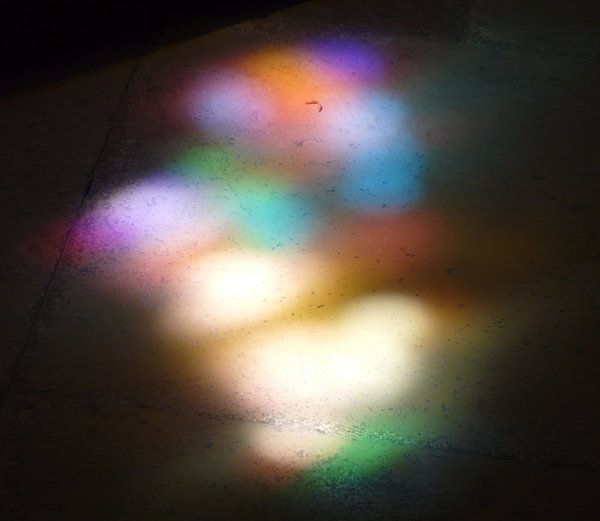
\includegraphics[width=\linewidth]{lichtspiel.jpg}};\end{tcbcliptitle}}]
% \lipsum[1]
% \end{tcolorbox}
% \end{dispExample}
% \end{docEnvironment}

% %\clearpage
% \begin{docTcbKey}{clip title}{\colOpt{=true\textbar false}}{default |true|, initially |false|}
%   Sets the title to be clipped to the title area.
% \begin{dispExample}
% \tcbset{enhanced,width=5cm,colframe=red!50!white,coltitle=black,
%   colbacktitle=yellow!50!white}

% \begin{tcolorbox}[title=\mbox{This is a title which is unbreakable and far too long}]
% This is a tcolorbox.
% \end{tcolorbox}

% \begin{tcolorbox}[title=\mbox{This is a title which is unbreakable and far too long},
%   clip title]
% This is a tcolorbox.
% \end{tcolorbox}
% \end{dispExample}
% \end{docTcbKey}


% \begin{docTcbKey}{clip upper}{\colOpt{=true\textbar false}}{default |true|, initially |false|}
%   Sets the upper part to be clipped to the interior area.
% \begin{dispExample}
% \newcommand{\mygraphics}[2][]{%
%   \tcbox[enhanced,boxsep=0pt,top=0pt,bottom=0pt,left=0pt,
%     right=0pt,boxrule=0.4pt,drop fuzzy shadow,clip upper,
%     colback=black!75!white,toptitle=2pt,bottomtitle=2pt,nobeforeafter,
%     center title,fonttitle=\small\sffamily,title=\detokenize{#2}]
%   {\includegraphics[width=\the\dimexpr(\linewidth-4mm)/2\relax]{#2}}}

% \mygraphics{lichtspiel.jpg}\hfill
% \mygraphics{Basilica_5.png}
% \end{dispExample}
% \end{docTcbKey}

% %\clearpage
% The example for \refKey{/tcb/clip upper} sizes the box according to
% the dimensions of the picture. To do it the other way around, the watermark
% options provide an easy solution.
% \begin{dispExample}
% \newcommand{\mygraphics}[2][]{%
%   \tcbox[enhanced,capture=minipage,boxsep=0pt,top=0pt,bottom=0pt,left=0pt,
%     right=0pt,boxrule=0.4pt,drop fuzzy shadow,nobeforeafter,
%     colback=black!75!white,toptitle=2pt,bottomtitle=2pt,
%     center title,fonttitle=\small\sffamily,title=\detokenize{#2},
%     width=(\linewidth-4mm)/2,height=6cm,colbacktitle={black},
%     watermark zoom=1.0,watermark graphics={#2}]{}}

% \mygraphics{lichtspiel.jpg}\hfill
% \mygraphics{Basilica_5.png}
% \end{dispExample}


% \begin{docTcbKey}{clip lower}{\colOpt{=true\textbar false}}{default |true|, initially |false|}
%   Sets the lower part to be clipped to the interior area.
% \begin{dispExample}
% \tcbset{enhanced,width=5cm,colframe=red!50!black,text and listing}

% \begin{tcblisting}{}
% Donau\-dampf\-schiff\-fahrts\-ka\-pi\-t\"ans\-m\"ut\-zen\-fran\-sen
% \end{tcblisting}

% \begin{tcblisting}{clip lower}
% Donau\-dampf\-schiff\-fahrts\-ka\-pi\-t\"ans\-m\"ut\-zen\-fran\-sen
% \end{tcblisting}
% \end{dispExample}
% \end{docTcbKey}


% %\clearpage
% \subsection{Border Line Option Keys}\label{subsec:borderline}
% The following borderline options are applicable for most skins which
% use |tikzpicture| as \refKey{/tcb/graphical environment}.
% Therefore, the skin \refSkin{standard} does not support these border lines,
% but most other skins, e.\,g.\ \refSkin{enhanced}.

% The borderlines are independent from the normal |tcolorbox| rules.
% They may be used with or without the \refKey{/tcb/segmentation engine}.

% The borderlines are stackable, i.\,e.\ several different border lines can be
% used on the same |tcolorbox|. They are drawn \emph{after} the box frame and box
% interior and \emph{before} overlays or watermarks.

% \begin{marker}
% Technically, the normal |tcolorbox| rules result from a \tikzname\  \emph{filling}
% process. The border lines are created by a \tikzname\  \emph{drawing} process.
% This can be used to apply different effects.
% \end{marker}


% \begin{docTcbKey}{borderline}{=\marg{width}\marg{offset}\marg{options}}{no default, initially unset}
%   Adds a new borderline to the stack of border lines.
%   This border line is drawn with the given \meta{width} and gets an
%   \meta{offset} computed from the frame outline. A positive \meta{offset} value
%   moves the borderline inside the |tcolorbox| and a negative \meta{offset} value
%   moves it outside without changing the bounding box.\\
%   The border line is drawn along a \tikzname\  path with the given \tikzname\  \meta{options}.
%   Note that the \tikzname\  |line width| option should not be used here.\\
%   The border lines adapt to the rounded corners of the |tcolorbox|. An inside
%   borderline will switch to sharp corners if necessary, an outside borderline will
%   always be rounded except for \refKey{/tcb/sharp corners}.
% \begin{dispExample}
% \begin{tcolorbox}[enhanced,title=Rounded corners,fonttitle=\bfseries,boxsep=5pt,
%   arc=8pt,
%   borderline={0.5pt}{0pt}{red},
%   borderline={0.5pt}{5pt}{blue,dotted},
%   borderline={0.5pt}{-5pt}{green} ]
% This is a tcolorbox.
% \end{tcolorbox}
% \bigskip
% \begin{tcolorbox}[enhanced,title=Sharp corners,fonttitle=\bfseries,boxsep=5pt,
%   arc=8pt,sharp corners=downhill,
%   borderline={0.5pt}{0pt}{red},
%   borderline={0.5pt}{5pt}{blue,dotted},
%   borderline={0.5pt}{-5pt}{green} ]
% This is a tcolorbox.
% \end{tcolorbox}
% \end{dispExample}

% \begin{dispExample}
% % \usepackage{lipsum}
% \begin{tcolorbox}[enhanced,arc=3mm,boxrule=1.5mm,boxsep=1.5mm,
%   colback=yellow!20!white,
%   colframe=blue,
%   borderline={1mm}{1mm}{white},
%   borderline={1mm}{2mm}{red} ]
%   \lipsum[1]
% \end{tcolorbox}
% \end{dispExample}


% \begin{dispExample}
% % \usepackage{lipsum}
% \begin{tcolorbox}[enhanced,arc=3mm,boxrule=1.5mm,
%   frame hidden,colback=blue!10!white,
%   borderline={1mm}{0mm}{blue,dotted} ]
%   \lipsum[2]
% \end{tcolorbox}
% \end{dispExample}


% \begin{dispExample}
% % \usepackage{lipsum}
% \begin{tcolorbox}[enhanced,skin=enhancedmiddle,
%   frame hidden,interior hidden,top=0mm,bottom=0mm,boxsep=0mm,
%   borderline={0.75mm}{0mm}{red},
%   borderline={0.75mm}{0.75mm}{red!50!yellow},
%   borderline={0.75mm}{1.5mm}{yellow}, ]
%   \lipsum[3]
% \end{tcolorbox}
% \end{dispExample}

% \begin{dispExample}
% % \usepackage{lipsum}
% \newtcolorbox{mygreenbox}[2][]{%
%   enhanced,width=\linewidth-6pt,
%   enlarge top by=3pt,enlarge bottom by=3pt,
%   enlarge left by=3pt,enlarge right by=3pt,
%   title={#2},frame hidden,boxrule=0pt,top=1mm,bottom=1mm,
%   colframe=green!30!black, colbacktitle=green!50!yellow,
%   coltitle=black, colback=green!25!white,
%   borderline={0.5pt}{-0.5pt}{green!75!blue},
%   borderline={1pt}{-3pt}{green!50!blue},#1}

% \begin{mygreenbox}{My title}
%   \lipsum[4]
% \end{mygreenbox}
% \end{dispExample}
% \end{docTcbKey}


% \begin{docTcbKey}{no borderline}{}{no default, initially set}
%   Removes all borderlines if set before.
% \end{docTcbKey}


% \begin{docTcbKey}{show bounding box}{\colOpt{=\meta{color}}}{default |red|, initially unset}
%   Displays the bounding box borderline of a |tcolorbox|.
%   Its intended use is debugging and fine tuning.
%   It should not be part of a final document.
%   The optional \meta{color} is the base color for the bounding box
%   borderline.
% \begin{dispExample}
% \tcbset{enhanced,nobeforeafter,width=4cm,fonttitle=\bfseries}

% \begin{tcolorbox}[show bounding box,title=Normal]
% This is a tcolorbox.
% \end{tcolorbox}%
% \begin{tcolorbox}[show bounding box=blue,title=Shadow,drop fuzzy shadow]
% This is a tcolorbox.
% \end{tcolorbox}%
% \begin{tcolorbox}[show bounding box=green,title=Enlarged,drop fuzzy shadow,
%   enlarge by=2mm]
% This is a tcolorbox.
% \end{tcolorbox}
% \end{dispExample}
% \end{docTcbKey}

% %\clearpage

% \begin{marker}
% The following \emph{partial} borderlines act slightly different from the
% complete borderlines described before. They ignore rounded corner settings,
% their length is not modified by their \meta{offset}, they ignore skin settings
% but adapt to breakable boxes.
% \end{marker}

% \begin{docTcbKey}[][doc new=2014-10-20]{borderline north}{=\marg{width}\marg{offset}\marg{options}}{no default, initially unset}
%   Adds a new borderline with the given \meta{width} to the
%   north of the |tcolorbox|.
%   A positive \meta{offset} value
%   moves the borderline inside the |tcolorbox| and a negative \meta{offset} value
%   moves it outside without changing the bounding box.
% \begin{dispExample*}{sbs,lefthand ratio=0.6}
% \begin{tcolorbox}[enhanced,
%   borderline north={2pt}{-2pt}{red}]
%   This is a \textbf{tcolorbox}.
% \end{tcolorbox}
% \end{dispExample*}
% \end{docTcbKey}

% \begin{docTcbKey}[][doc new=2014-10-20]{borderline south}{=\marg{width}\marg{offset}\marg{options}}{no default, initially unset}
%   Adds a new borderline with the given \meta{width} to the
%   south of the |tcolorbox|.
%   A positive \meta{offset} value
%   moves the borderline inside the |tcolorbox| and a negative \meta{offset} value
%   moves it outside without changing the bounding box.
% \begin{dispExample*}{sbs,lefthand ratio=0.6}
% \begin{tcolorbox}[enhanced,
%   borderline south={2pt}{-2pt}{red}]
%   This is a \textbf{tcolorbox}.
% \end{tcolorbox}
% \end{dispExample*}
% \end{docTcbKey}

% \begin{docTcbKey}[][doc new=2014-10-20]{borderline east}{=\marg{width}\marg{offset}\marg{options}}{no default, initially unset}
%   Adds a new borderline with the given \meta{width} to the
%   east of the |tcolorbox|.
%   A positive \meta{offset} value
%   moves the borderline inside the |tcolorbox| and a negative \meta{offset} value
%   moves it outside without changing the bounding box.
% \begin{dispExample*}{sbs,lefthand ratio=0.6}
% \begin{tcolorbox}[enhanced,
%   borderline east={2pt}{-2pt}{red}]
%   This is a \textbf{tcolorbox}.
% \end{tcolorbox}
% \end{dispExample*}
% \end{docTcbKey}

% \begin{docTcbKey}[][doc new=2014-10-20]{borderline west}{=\marg{width}\marg{offset}\marg{options}}{no default, initially unset}
%   Adds a new borderline with the given \meta{width} to the
%   west of the |tcolorbox|.
%   A positive \meta{offset} value
%   moves the borderline inside the |tcolorbox| and a negative \meta{offset} value
%   moves it outside without changing the bounding box.
% \begin{dispExample*}{sbs,lefthand ratio=0.6}
% \begin{tcolorbox}[enhanced,
%   borderline west={2pt}{-2pt}{red}]
%   This is a \textbf{tcolorbox}.
% \end{tcolorbox}
% \end{dispExample*}
% \end{docTcbKey}

% %\clearpage
% \begin{docTcbKey}[][doc new=2014-10-20]{borderline horizontal}{=\marg{width}\marg{offset}\marg{options}}{no default, initially unset}
%   Adds a new borderline with the given \meta{width} to the
%   north and south of the |tcolorbox|.
%   A positive \meta{offset} value
%   moves the borderlines inside the |tcolorbox| and a negative \meta{offset} value
%   moves them outside without changing the bounding box.
% \begin{dispExample*}{sbs,lefthand ratio=0.6}
% \begin{tcolorbox}[blanker,top=3mm,bottom=3mm,
%    borderline horizontal={2pt}{0pt}{red}]
%   This is a \textbf{tcolorbox}.
% \end{tcolorbox}
% \end{dispExample*}
% \end{docTcbKey}


% \begin{docTcbKey}[][doc new=2014-10-20]{borderline vertical}{=\marg{width}\marg{offset}\marg{options}}{no default, initially unset}
%   Adds a new borderline with the given \meta{width} to the
%   east and west of the |tcolorbox|.
%   A positive \meta{offset} value
%   moves the borderlines inside the |tcolorbox| and a negative \meta{offset} value
%   moves them outside without changing the bounding box.
% \begin{dispExample*}{sbs,lefthand ratio=0.6}
% \begin{tcolorbox}[blanker,left=3mm,right=3mm,
%    borderline vertical={2pt}{0pt}{red}]
%   This is a \textbf{tcolorbox}.\\
%   My second line.
% \end{tcolorbox}
% \end{dispExample*}
% \end{docTcbKey}

% \begin{dispExample}
% \begin{tcolorbox}[enhanced,colback=yellow!10!white,boxrule=0pt,frame hidden,
%   borderline north={1mm}{-2mm}{red},
%   borderline south={1mm}{-2mm}{blue},
%   borderline west={1mm}{-2mm}{green},
%   borderline east={1mm}{-2mm}{yellow}]
% \lipsum[1]
% \end{tcolorbox}
% \end{dispExample}

% %\clearpage
% \subsection{Shadow Option Keys}\label{subsec:shadows}
% The following shadow options are applicable for most skins which
% use |tikzpicture| as \refKey{/tcb/graphical environment}.
% Therefore, the skin \refSkin{standard} does not support these shadows,
% but most other skins, e.\,g.\ \refSkin{enhanced}.

% The shadows are stackable, i.\,e.\ several different shadows can be
% used on the same |tcolorbox|. They are drawn \emph{before} the box frame is drawn.

% \begin{docTcbKey}{no shadow}{}{no default}
%   Removes all shadows if set before.
% \end{docTcbKey}

% \subsubsection{Common Shadows and Halos}

% \begin{docTcbKey}{drop shadow}{\colOpt{=\meta{color}}}{style, default |black!50!white|}
%   Adds a new shadow with standard dimensions to the stack of shadows.
%   Optionally, the \meta{color} for the shadow can be changed.
% \begin{dispExample*}{sbs,lefthand ratio=0.6}
% \tcbset{enhanced,colback=red!5!white,
%   colframe=red!75!black,fonttitle=\bfseries}

% \begin{tcolorbox}[drop shadow]
% This is a tcolorbox.
% \end{tcolorbox}\par\bigskip
% \begin{tcolorbox}[title=Another shadow,
%   drop shadow=blue]
% This is a tcolorbox.
% \end{tcolorbox}
% \end{dispExample*}
% \end{docTcbKey}


% \begin{docTcbKey}{drop fuzzy shadow}{\colOpt{=\meta{color}}}{style, default |black!50!white|}
%   Adds a new fuzzy shadow with standard dimensions to the stack of shadows.
%   Optionally, the \meta{color} for the shadow can be changed.
% \begin{dispExample*}{sbs,lefthand ratio=0.6}
% \tcbset{enhanced,colback=red!5!white,
%   colframe=red!75!black,fonttitle=\bfseries}

% \begin{tcolorbox}[drop fuzzy shadow]
% This is a tcolorbox.
% \end{tcolorbox}\par\bigskip
% \begin{tcolorbox}[title=Another shadow,
%   drop fuzzy shadow=blue]
% This is a tcolorbox.
% \end{tcolorbox}
% \end{dispExample*}
% \end{docTcbKey}


% \begin{docTcbKey}{drop midday shadow}{\colOpt{=\meta{color}}}{style, default |black!50!white|}
%   Adds a new shadow with standard dimensions to the stack of shadows.
%   Optionally, the \meta{color} for the shadow can be changed.
% \begin{dispExample*}{sbs,lefthand ratio=0.6}
% \tcbset{enhanced,colback=red!5!white,
%   colframe=red!75!black,fonttitle=\bfseries}

% \begin{tcolorbox}[drop midday shadow]
% This is a tcolorbox.
% \end{tcolorbox}\par\bigskip
% \begin{tcolorbox}[title=Another shadow,
%   drop midday shadow=blue]
% This is a tcolorbox.
% \end{tcolorbox}
% \end{dispExample*}
% \end{docTcbKey}

% %\enlargethispage*{2cm}
% \begin{docTcbKey}{drop fuzzy midday shadow}{\colOpt{=\meta{color}}}{style, default |black!50!white|}
%   Adds a new fuzzy shadow with standard dimensions to the stack of shadows.
%   Optionally, the \meta{color} for the shadow can be changed.
% \begin{dispExample*}{sbs,lefthand ratio=0.6}
% \tcbset{enhanced,colback=red!5!white,
%   colframe=red!75!black,fonttitle=\bfseries}

% \begin{tcolorbox}[drop fuzzy midday shadow]
% This is a tcolorbox.
% \end{tcolorbox}\par\bigskip
% \begin{tcolorbox}[title=Another shadow,
%   drop fuzzy midday shadow=blue]
% This is a tcolorbox.
% \end{tcolorbox}
% \end{dispExample*}
% \end{docTcbKey}


% \begin{docTcbKey}{halo}{\colOpt{=\meta{size} \texttt{with} \meta{color}}}{style, default |0.9mm with yellow|}
%   Adds a new halo shadow with the given \meta{color}
%   which overlaps the colorbox an all sides by \meta{size}.
% \begin{dispExample*}{sbs,lefthand ratio=0.6}
% \tcbset{enhanced,colback=red!5!white,
%   colframe=red!75!black,fonttitle=\bfseries}

% \begin{tcolorbox}[title=My own halo,halo]
% This is a tcolorbox.
% \end{tcolorbox}
% \par\bigskip\bigskip
% \begin{tcolorbox}[title=Another halo,
%   halo=2mm with green]
% This is a tcolorbox.
% \end{tcolorbox}
% \end{dispExample*}
% \end{docTcbKey}

% \enlargethispage*{2cm}
% \begin{docTcbKey}{fuzzy halo}{\colOpt{=\meta{size} \texttt{with} \meta{color}}}{style, default |0.9mm with yellow|}
%   Adds a new fuzzy halo shadow with the given \meta{color}
%   which overlaps the colorbox an all sides by \meta{size} plus |0.48mm|.
% \begin{dispExample*}{sbs,lefthand ratio=0.6}
% \tcbset{enhanced,colback=red!5!white,
%   colframe=red!75!black,fonttitle=\bfseries}

% \begin{tcolorbox}[title=My own halo,fuzzy halo]
% This is a tcolorbox.
% \end{tcolorbox}
% \par\bigskip\bigskip
% \begin{tcolorbox}[title=Another halo,
%   fuzzy halo=2mm with green]
% This is a tcolorbox.
% \end{tcolorbox}
% \end{dispExample*}

% \begin{dispExample}
% \begin{tcolorbox}[blank,enhanced jigsaw,boxsep=2pt,arc=2pt,
%   fuzzy halo=2mm with red!50!white,
%   fuzzy halo=1mm with white]
% \lipsum[1]
% \end{tcolorbox}
% \end{dispExample}
% \end{docTcbKey}


% %\clearpage
% For all following shadows, the optionally given \meta{color} for the shadow can be changed
% equivalent to the preceding examples.

% \begin{docTcbKey}{drop shadow southeast}{\colOpt{=\meta{color}}}{style, default |black!50!white|}
%   Adds a new shadow with standard dimensions to the stack of shadows.
%   This shadow is identical to \refKey{/tcb/drop shadow}.
% \begin{dispExample*}{sbs,lefthand ratio=0.7}
% \begin{tcolorbox}[drop shadow southeast,
%   enhanced,colback=red!5!white,colframe=red!75!black]
%   This is a tcolorbox.
% \end{tcolorbox}
% \end{dispExample*}
% \end{docTcbKey}%

% \begin{docTcbKey}{drop shadow south}{\colOpt{=\meta{color}}}{style, default |black!50!white|}
%   Adds a new shadow with standard dimensions to the stack of shadows.
%   This shadow is identical to \refKey{/tcb/drop midday shadow}.
% \begin{dispExample*}{sbs,lefthand ratio=0.7}
% \begin{tcolorbox}[drop shadow south,
%   enhanced,colback=red!5!white,colframe=red!75!black]
%   This is a tcolorbox.
% \end{tcolorbox}
% \end{dispExample*}
% \end{docTcbKey}%

% \begin{docTcbKey}{drop shadow southwest}{\colOpt{=\meta{color}}}{style, default |black!50!white|}
%   Adds a new shadow with standard dimensions to the stack of shadows.
% \begin{dispExample*}{sbs,lefthand ratio=0.7}
% \begin{tcolorbox}[drop shadow southwest,
%   enhanced,colback=red!5!white,colframe=red!75!black]
%   This is a tcolorbox.
% \end{tcolorbox}
% \end{dispExample*}
% \end{docTcbKey}%

% \begin{docTcbKey}{drop shadow west}{\colOpt{=\meta{color}}}{style, default |black!50!white|}
%   Adds a new shadow with standard dimensions to the stack of shadows.
% \begin{dispExample*}{sbs,lefthand ratio=0.7}
% \begin{tcolorbox}[drop shadow west,
%   enhanced,colback=red!5!white,colframe=red!75!black]
%   This is a tcolorbox.
% \end{tcolorbox}
% \end{dispExample*}
% \end{docTcbKey}%

% \begin{docTcbKey}{drop shadow northwest}{\colOpt{=\meta{color}}}{style, default |black!50!white|}
%   Adds a new shadow with standard dimensions to the stack of shadows.
% \begin{dispExample*}{sbs,lefthand ratio=0.7}
% \begin{tcolorbox}[drop shadow northwest,
%   enhanced,colback=red!5!white,colframe=red!75!black]
%   This is a tcolorbox.
% \end{tcolorbox}
% \end{dispExample*}
% \end{docTcbKey}%

% \begin{docTcbKey}{drop shadow north}{\colOpt{=\meta{color}}}{style, default |black!50!white|}
%   Adds a new shadow with standard dimensions to the stack of shadows.
% \begin{dispExample*}{sbs,lefthand ratio=0.7}
% \begin{tcolorbox}[drop shadow north,
%   enhanced,colback=red!5!white,colframe=red!75!black]
%   This is a tcolorbox.
% \end{tcolorbox}
% \end{dispExample*}
% \end{docTcbKey}%

% %\clearpage
% \begin{docTcbKey}{drop shadow northeast}{\colOpt{=\meta{color}}}{style, default |black!50!white|}
%   Adds a new shadow with standard dimensions to the stack of shadows.
% \begin{dispExample*}{sbs,lefthand ratio=0.7}
% \begin{tcolorbox}[drop shadow northeast,
%   enhanced,colback=red!5!white,colframe=red!75!black]
%   This is a tcolorbox.
% \end{tcolorbox}
% \end{dispExample*}
% \end{docTcbKey}%

% \begin{docTcbKey}{drop shadow east}{\colOpt{=\meta{color}}}{style, default |black!50!white|}
%   Adds a new shadow with standard dimensions to the stack of shadows.
% \begin{dispExample*}{sbs,lefthand ratio=0.7}
% \begin{tcolorbox}[drop shadow east,
%   enhanced,colback=red!5!white,colframe=red!75!black]
%   This is a tcolorbox.
% \end{tcolorbox}
% \end{dispExample*}
% \end{docTcbKey}%


% \begin{docTcbKey}{drop fuzzy shadow southeast}{\colOpt{=\meta{color}}}{style, default |black!50!white|}
%   Adds a new fuzzy shadow with standard dimensions to the stack of shadows.
%   This shadow is identical to \refKey{/tcb/drop fuzzy shadow}.
% \begin{dispExample*}{sbs,lefthand ratio=0.7}
% \begin{tcolorbox}[drop fuzzy shadow southeast,
%   enhanced,colback=red!5!white,colframe=red!75!black]
%   This is a tcolorbox.
% \end{tcolorbox}
% \end{dispExample*}
% \end{docTcbKey}%

% \begin{docTcbKey}{drop fuzzy shadow south}{\colOpt{=\meta{color}}}{style, default |black!50!white|}
%   Adds a new fuzzy shadow with standard dimensions to the stack of shadows.
%   This shadow is identical to \refKey{/tcb/drop fuzzy midday shadow}.
% \begin{dispExample*}{sbs,lefthand ratio=0.7}
% \begin{tcolorbox}[drop fuzzy shadow south,
%   enhanced,colback=red!5!white,colframe=red!75!black]
%   This is a tcolorbox.
% \end{tcolorbox}
% \end{dispExample*}
% \end{docTcbKey}%

% \begin{docTcbKey}{drop fuzzy shadow southwest}{\colOpt{=\meta{color}}}{style, default |black!50!white|}
%   Adds a new fuzzy shadow with standard dimensions to the stack of shadows.
% \begin{dispExample*}{sbs,lefthand ratio=0.7}
% \begin{tcolorbox}[drop fuzzy shadow southwest,
%   enhanced,colback=red!5!white,colframe=red!75!black]
%   This is a tcolorbox.
% \end{tcolorbox}
% \end{dispExample*}
% \end{docTcbKey}%

% \begin{docTcbKey}{drop fuzzy shadow west}{\colOpt{=\meta{color}}}{style, default |black!50!white|}
%   Adds a new fuzzy shadow with standard dimensions to the stack of shadows.
% \begin{dispExample*}{sbs,lefthand ratio=0.7}
% \begin{tcolorbox}[drop fuzzy shadow west,
%   enhanced,colback=red!5!white,colframe=red!75!black]
%   This is a tcolorbox.
% \end{tcolorbox}
% \end{dispExample*}
% \end{docTcbKey}%

% %\clearpage
% \begin{docTcbKey}{drop fuzzy shadow northwest}{\colOpt{=\meta{color}}}{style, default |black!50!white|}
%   Adds a new fuzzy shadow with standard dimensions to the stack of shadows.
% \begin{dispExample*}{sbs,lefthand ratio=0.7}
% \begin{tcolorbox}[drop fuzzy shadow northwest,
%   enhanced,colback=red!5!white,colframe=red!75!black]
%   This is a tcolorbox.
% \end{tcolorbox}
% \end{dispExample*}
% \end{docTcbKey}%

% \begin{docTcbKey}{drop fuzzy shadow north}{\colOpt{=\meta{color}}}{style, default |black!50!white|}
%   Adds a new fuzzy shadow with standard dimensions to the stack of shadows.
% \begin{dispExample*}{sbs,lefthand ratio=0.7}
% \begin{tcolorbox}[drop fuzzy shadow north,
%   enhanced,colback=red!5!white,colframe=red!75!black]
%   This is a tcolorbox.
% \end{tcolorbox}
% \end{dispExample*}
% \end{docTcbKey}%

% \begin{docTcbKey}{drop fuzzy shadow northeast}{\colOpt{=\meta{color}}}{style, default |black!50!white|}
%   Adds a new fuzzy shadow with standard dimensions to the stack of shadows.
% \begin{dispExample*}{sbs,lefthand ratio=0.7}
% \begin{tcolorbox}[drop fuzzy shadow northeast,
%   enhanced,colback=red!5!white,colframe=red!75!black]
%   This is a tcolorbox.
% \end{tcolorbox}
% \end{dispExample*}
% \end{docTcbKey}%

% \begin{docTcbKey}{drop fuzzy shadow east}{\colOpt{=\meta{color}}}{style, default |black!50!white|}
%   Adds a new fuzzy shadow with standard dimensions to the stack of shadows.
% \begin{dispExample*}{sbs,lefthand ratio=0.7}
% \begin{tcolorbox}[drop fuzzy shadow east,
%   enhanced,colback=red!5!white,colframe=red!75!black]
%   This is a tcolorbox.
% \end{tcolorbox}
% \end{dispExample*}
% \end{docTcbKey}%


% %\clearpage
% \subsubsection{Lifted Shadows}

% \begin{docTcbKey}{drop lifted shadow}{\colOpt{=\meta{color}}}{style, default |black!50!white|}
%   Adds a new lifted shadow with standard dimensions to the stack of shadows.
%   Optionally, the \meta{color} for the shadow can be changed.
% \begin{dispExample*}{sbs,lefthand ratio=0.6}
% \tcbset{enhanced,colback=red!5!white,
%   boxrule=0.4pt,sharp corners,
%   colframe=red!75!black,fonttitle=\bfseries}

% \begin{tcolorbox}[drop lifted shadow]
% This is a tcolorbox.
% \end{tcolorbox}\par\bigskip
% \begin{tcolorbox}[title=Another shadow,
%   drop lifted shadow=blue]
% This is a tcolorbox.
% \end{tcolorbox}
% \end{dispExample*}
% \end{docTcbKey}


% \begin{docTcbKey}{drop small lifted shadow}{\colOpt{=\meta{color}}}{style, default |black!50!white|}
%   Adds a new small lifted shadow with standard dimensions to the stack of shadows.
%   Optionally, the \meta{color} for the shadow can be changed.
% \begin{dispExample*}{sbs,lefthand ratio=0.6}
% \tcbset{enhanced,colback=red!5!white,
%   boxrule=0.4pt,sharp corners,
%   colframe=red!75!black,fonttitle=\bfseries}

% \tcbox[drop small lifted shadow,size=fbox]
%   {This is a tcolorbox.}
% \par\bigskip
% \begin{tcolorbox}[title=Another shadow,
%   drop small lifted shadow=black]
% This is a tcolorbox.
% \end{tcolorbox}
% \end{dispExample*}
% \end{docTcbKey}


% \begin{docTcbKey}{drop large lifted shadow}{\colOpt{=\meta{color}}}{style, default |black!50!white|}
%   Adds a new large lifted shadow with standard dimensions to the stack of shadows.
%   Optionally, the \meta{color} for the shadow can be changed.
% \begin{dispExample*}{sbs,lefthand ratio=0.6}
% \tcbset{enhanced,colback=red!5!white,
%   colframe=red!75!black,fonttitle=\bfseries}

% \begin{tcolorbox}[drop large lifted shadow]
% This is a tcolorbox.
% \end{tcolorbox}\par\bigskip
% \begin{tcolorbox}[title=Another shadow,
%   drop large lifted shadow=blue]
% This is a tcolorbox.
% \end{tcolorbox}
% \end{dispExample*}
% \end{docTcbKey}


% %\clearpage

% \subsubsection{Generic Shadows}
% \begin{docTcbKey}{shadow}{=\marg{xshift}\marg{yshift}\marg{offset}\marg{options}}{no default}
%   Adds a new shadow to the stack of shadows.
%   This shadow follows the outline of the |tcolorbox| but is shifted by
%   \meta{xshift} and \meta{yshift}. The \meta{offset} value is a distance value
%   from the frame outline.  A positive \meta{offset} value shrinks the shadow
%   and a negative \meta{offset} value enlarges the shadow.
%   The shadow is filled along a \tikzname\  path with the given \tikzname\  \meta{options}.\\
%   The shadows adapt to the rounded corners of the |tcolorbox|. An shrinked shadow
%   will switch to sharp corners if necessary, an enlarged shadow may become
%   more rounded depending on several factors. But \refKey{/tcb/sharp corners}
%   have sharp shadows.
%   \begin{marker}
%   Shadows are not considered for the bounding box computation by default.
%   Large shadows may be overlaped by the following content. But, the
%   bounding box can be adapted if necessary.
%   \end{marker}

% \begin{dispExample*}{sbs,lefthand ratio=0.6}
% \tcbset{enhanced,colback=red!5!white,
%   colframe=red!75!black,fonttitle=\bfseries}

% \begin{tcolorbox}[title=My own shadow,
%   shadow={2mm}{-1mm}{0mm}{black!50!white}]
% This is a tcolorbox.
% \end{tcolorbox}
% \par\bigskip
% \begin{tcolorbox}[title=Another shadow,
%   shadow={-1mm}{-2mm}{0mm}{fill=blue,
%     opacity=0.5}]
% This is a tcolorbox.
% \end{tcolorbox}
% \par\bigskip
% \begin{tcolorbox}[title=Double shadow,
%   shadow={-1.5mm}{-1.5mm}{0mm}{fill=blue,
%     opacity=0.25},
%   shadow={1.5mm}{-1.5mm}{0mm}{fill=red,
%     opacity=0.25}]
% This is a tcolorbox.
% \end{tcolorbox}
% \par\bigskip
% \begin{tcolorbox}[title=Far shadow,
%   shadow={5.5mm}{-3.5mm}{2mm}{fill=black,
%     opacity=0.25}]
% This is a tcolorbox.
% \end{tcolorbox}
% \par\bigskip\bigskip
% \begin{tcolorbox}[title=Halo shadow,
%   shadow={0mm}{0mm}{-1.5mm}%
%      {fill=yellow!75!red,opacity=0.5}]
% This is a tcolorbox.
% \end{tcolorbox}
% \end{dispExample*}
% \end{docTcbKey}

% %\clearpage
% \begin{docTcbKey}{fuzzy shadow}{=\marg{xshift}\marg{yshift}\marg{offset}\marg{step}\marg{options}}{no default}
%   Adds a new fuzzy shadow to the stack of shadows. Actually, this option
%   adds several shadows which appear like a shadow with a fuzzy border.
%   This fuzzy shadow follows the outline of the |tcolorbox| but is shifted by
%   \meta{xshift} and \meta{yshift}. The \meta{offset} value is a distance value
%   from the frame outline.  A positive \meta{offset} value shrinks the shadow
%   and a negative \meta{offset} value enlarges the shadow.
%   The \marg{step} value describes a shrink
%   offset used for the combination of the partial shadows.
%   The shadow is filled along a \tikzname\  path with the given \tikzname\  \meta{options} but
%   any |opacity| value will be ignored.
% \begin{dispExample*}{sbs,lefthand ratio=0.6}
% \tcbset{enhanced,colback=red!5!white,
%   colframe=red!75!black,fonttitle=\bfseries}

% \begin{tcolorbox}[title=My own shadow,
%   fuzzy shadow={2mm}{-1mm}{0mm}{0.1mm}%
%                {black!50!white}]
% This is a tcolorbox.
% \end{tcolorbox}
% \par\bigskip
% \begin{tcolorbox}[title=Another shadow,
%   fuzzy shadow={-1mm}{-2mm}{0mm}{0.2mm}%
%                {fill=blue}]
% This is a tcolorbox.
% \end{tcolorbox}
% \par\bigskip
% \begin{tcolorbox}[title=Double shadow,
%   fuzzy shadow={-1.5mm}{-1.5mm}{0mm}{0.1mm}%
%                {blue},
%   fuzzy shadow={1.5mm}{-1.5mm}{0mm}{0.1mm}%
%                {red}]
% This is a tcolorbox.
% \end{tcolorbox}
% \par\bigskip
% \begin{tcolorbox}[title=Far shadow,
%   fuzzy shadow={5.5mm}{-3.5mm}{0mm}{0.3mm}%
%                {black}]
% This is a tcolorbox.
% \end{tcolorbox}
% \par\bigskip\bigskip
% \begin{tcolorbox}[title=Glow shadow,
%   fuzzy shadow={0mm}{0mm}{-1.5mm}{0.15mm}%
%                {yellow!75!red}]
% This is a tcolorbox.
% \end{tcolorbox}
% \end{dispExample*}

% \begin{dispExample}
% \newtcolorbox{mybox}[1][]{enhanced,
%   fuzzy shadow={1.0mm}{-1.0mm}{0.12mm}{0mm}{blue!50!white},
%   fuzzy shadow={-1.0mm}{-1.0mm}{0.12mm}{0mm}{red!50!white},
%   fuzzy shadow={-1.0mm}{1.0mm}{0.12mm}{0mm}{green!50!white},
%   fuzzy shadow={1.0mm}{1.0mm}{0.12mm}{0mm}{yellow!50!white},#1
% }

% \begin{mybox}[title=A multi shadow box]
% This is a tcolorbox.
% \end{mybox}
% \end{dispExample}
% \end{docTcbKey}


% %\clearpage
% \begin{docTcbKey}[][doc new=2015-05-05]{smart shadow arc}{\colOpt{=true\textbar false}}{default |true|,
%   initially |true|}
% If set to |true|, the shadow drawing algorithm tries to do a somewhat
% smart calculation of the arc for the shadow. The result is pleasing for typical boxes
% with rounded corners, but gives strange results for circular boxes.

% \begin{dispExample}
% \tcbset{enhanced,nobeforeafter,colback=red!5!white,
%   colframe=red!75!black,width=3cm,square,halign=center,valign=center
%   }

% \begin{tcolorbox}[drop shadow]
% Smart shadow arc (arguably better than normal)
% \end{tcolorbox}
% \hfill
% \begin{tcolorbox}[smart shadow arc=false, drop shadow]
% Normal shadow arc
% \end{tcolorbox}
% \hfill
% \begin{tcolorbox}[circular arc, drop shadow]
% Smart shadow arc (worse than normal)
% \end{tcolorbox}
% \hfill
% \begin{tcolorbox}[circular arc, smart shadow arc=false, drop shadow]
% Normal shadow arc
% \end{tcolorbox}
% \end{dispExample}
% \end{docTcbKey}


% \begin{docTcbKey}{lifted shadow}{=\marg{xshift}\marg{yshift}\marg{bend}\marg{step}\marg{options}}{no default}
%   Adds a new lifted shadow to the stack of shadows. Actually, this option
%   adds several shadows which appear like a shadow with a fuzzy border.
%   This lifted shadow follows the outline of the |tcolorbox| but is shifted by
%   \meta{xshift} and \meta{yshift} on the lower left corner and by
%   $-$\meta{xshift} and \meta{yshift} on the lower right corner.
%   Additionally, there is a \meta{bend} in the middle.
%   The \marg{step} value describes a shrink
%   offset used for the combination of the partial shadows.
%   The shadow is filled along a \tikzname\  path with the given \tikzname\  \meta{options} but
%   any |opacity| value will be ignored.
% \begin{dispExample*}{sbs,lefthand ratio=0.6}
% \tcbset{enhanced,colback=red!5!white,
%   boxrule=0.1pt,
%   colframe=red!75!black,fonttitle=\bfseries}

% \begin{tcolorbox}[title=My own shadow,
%   lifted shadow={1mm}{-2mm}{3mm}{0.1mm}%
%                {black!50!white}]
% This is a tcolorbox.
% \end{tcolorbox}
% \end{dispExample*}
% \end{docTcbKey}

% %\clearpage
% \subsubsection{\tikzname\ Shadows}
% Alternativ to the package shadow options described before, shadows from
% the \flqq Shadows Library\frqq\ of \tikzname\ can be used.
% Such shadows can be added directly to the frame path using \refKey{/tcb/frame style}.

% \begin{exdispExample*}{tikz_shadow_1}{sbs,lefthand ratio=0.7}
% % \usetikzlibrary{shadows}
% \begin{tcolorbox}[enhanced,
%   colback=red!5!white,colframe=red!75!black,
%   frame style={drop shadow} ]
%   This is a tcolorbox.
% \end{tcolorbox}
% \end{exdispExample*}

% \begin{exdispExample*}{tikz_shadow_2}{sbs,lefthand ratio=0.7}
% % \usetikzlibrary{shadows}
% \begin{tcolorbox}[enhanced,height=3cm,
%   colback=red!5!white,colframe=red!75!black,
%   halign=center,valign=center,
%   frame style={circular drop shadow} ]
%   This is a tcolorbox.
% \end{tcolorbox}
% \end{exdispExample*}

% \begin{exdispExample*}{tikz_shadow_3}{sbs,lefthand ratio=0.7}
% % \usetikzlibrary{shadows}
% \begin{tcolorbox}[enhanced,width=2.5cm,
%   square,circular arc,
%   halign=center,valign=center,
%   colback=red!5!white,colframe=red!75!black,
%   frame style={circular glow={fill=red}} ]
%   tcolorbox
% \end{tcolorbox}
% \end{exdispExample*}


% %\clearpage
% \subsection{\tikzname\  Picture Option Keys}\label{subsec:tikzpicture}
% The following general options are applicable for skins which
% use |tikzpicture| as \refKey{/tcb/graphical environment}.
% Therefore, the skin \refSkin{standard} does not support these options,
% but most other skins, e.\,g.\ \refSkin{enhanced}.


% \begin{docTcbKey}{tikz}{=\meta{tikz option list}}{no default, initially empty}
%   Adds the given \meta{tikz option list} to the main |tikzpicture| environment
%   used to draw the color box, see \cite{tantau:tikz_and_pgf}. If this option is
%   applied a second time, the new \meta{tikz option list} is appended to the
%   current option list.
% \begin{dispExample*}{sbs,lefthand ratio=0.66,
%   segmentation style={preaction={fill=white},pattern=checkerboard,pattern color=gray!40}}
% \tcbset{enhanced,colback=red!5!white,
%   colframe=red!75!black,fonttitle=\bfseries}

% \begin{tcolorbox}[title=Transparent box,
%   tikz={opacity=0.5,transparency group}]
% This is a tcolorbox.
% \end{tcolorbox}
% \end{dispExample*}

% \begin{dispExample*}{sbs,lefthand ratio=0.66}
% \tcbset{enhanced,colback=red!5!white,
%   colframe=red!75!black,fonttitle=\bfseries,
%   fontupper=\bfseries\Huge,
%   halign title=center,halign=center}

% \begin{tcolorbox}[title=Rotated box,
%   tikz={rotate=30}]
% Sold!
% \end{tcolorbox}
% \end{dispExample*}

% \end{docTcbKey}


% \begin{docTcbKey}{tikz reset}{}{initially set}
%   Removes all options given by \refKey{/tcb/tikz}.
% \end{docTcbKey}


% \begin{docTcbKey}{at begin tikz}{=\meta{tikz code}}{no default, initially empty}
%   The given \meta{tikz code} is executed at the beginning of the |tikzpicture| environment
%   after the \tikzname\  option |execute at begin picture| was applied.
%   If this option is applied a second time, the new \meta{tikz code} is appended to the current code.
% \end{docTcbKey}


% \begin{docTcbKey}{at begin tikz reset}{}{initially set}
%   Removes all code given by \refKey{/tcb/at begin tikz}.
% \end{docTcbKey}


% \begin{docTcbKey}{at end tikz}{=\meta{tikz code}}{no default, initially empty}
%   The given \meta{tikz code} is executed at the ending of the |tikzpicture| environment
%   before the \tikzname\  option |execute at end picture| was applied.
%   If this option is applied a second time, the new \meta{tikz code} is appended to the current code.
% \end{docTcbKey}


% \begin{docTcbKey}{at end tikz reset}{}{initially set}
%   Removes all code given by \refKey{/tcb/at end tikz}.
% \end{docTcbKey}


% %\clearpage
% \begin{docTcbKey}{rotate}{=\meta{angle}}{no default, initially unset}
%   Rotates the |tcolorbox| by the given \meta{angle}. Note that this is
%   a \tikzname\  coordinate transformation i.e. not all graphical elements like shadings
%   will really be rotated.
% \begin{dispExample*}{sbs,lefthand ratio=0.66}
% \tcbset{enhanced,colback=red!5!white,
%   colframe=red!75!black,fonttitle=\bfseries}

% \begin{tcolorbox}[title=Rotated box,rotate=30]
% This is a tcolorbox.
% \end{tcolorbox}
% \end{dispExample*}
% \end{docTcbKey}

% \begin{docTcbKey}{scale}{=\meta{fraction}}{no default, initially unset}
%   Scales the |tcolorbox| by the given \meta{fraction}. Note that this is
%   a \tikzname\  coordinate transformation i.e. not all graphical elements like line widths
%   will really be scaled.
% \begin{dispExample*}{sbs,lefthand ratio=0.66}
% \tcbset{enhanced,colback=red!5!white,
%   colframe=red!75!black,fonttitle=\bfseries}

% \begin{tcolorbox}[title=Scaled box,scale=0.5]
% This is a tcolorbox.
% \end{tcolorbox}
% \begin{tcolorbox}[title=Scaled box,scale=1.25]
% This is a tcolorbox.
% \end{tcolorbox}
% \end{dispExample*}
% \end{docTcbKey}


% \begin{docTcbKey}{remember}{}{style, initially unset}
%   Shortcut for |tikz={remember picture}|. This allows one to reference nodes
%   in other \tikzname\  pictures.
% \begin{dispExample}
% \begin{tcolorbox}[enhanced,remember,colback=red!5!white,colframe=red!75!black,
%   fonttitle=\bfseries,title=The four corners of a paper,
%   overlay={\draw[red!50!white,line width=1mm,opacity=0.5,shorten >=3mm]
%     (frame.north west) edge[->] (current page.north west)
%     (frame.north east) edge[->] (current page.north east)
%     (frame.south west) edge[->] (current page.south west)
%     (frame.south east) edge[->] (current page.south east);}]
% This is a tcolorbox.
% \end{tcolorbox}
% \end{dispExample}
% \end{docTcbKey}

% %\clearpage
% \tcbinterruptdraftmode%
% \begin{docTcbKey}{remember as}{=\meta{name}}{style, no default, initially unset}
%   The |frame| node will be remembered by the given \meta{name} to be referenced
%   in other \tikzname\  pictures.
% \begin{dispExample}
% % \usepackage{lipsum}
% \newtcolorbox{mybox}[1][]{enhanced,colframe=blue!75!black,colback=blue!10!white,
%   fonttitle=\bfseries,#1}

% \begin{mybox}[title=First Box,nobeforeafter,width=\linewidth/4,remember as=one]
% This is a test.
% \end{mybox}
% \hfill
% \begin{mybox}[title=Second Box,nobeforeafter,width=\linewidth/4,remember as=two]
% This is a test.
% \end{mybox}
% \hfill
% \begin{mybox}[title=Third Box,nobeforeafter,width=\linewidth/4,remember as=three]
% This is a test.
% \end{mybox}

% \lipsum[2]

% \begin{mybox}[title=Fourth Box,remember as=four]
% This is a test.
% \end{mybox}

% \begin{tikzpicture}[overlay,remember picture,line width=1mm,draw=red!75!black]
%   \draw[->] (one.east) to[bend right] node[above] {A} (two.west);
%   \draw[->] (two.east) to[bend left] node[above] {B} (three.west);
%   \draw[->] (three.east) to[bend left=90] node[right] {C} (four.east);
%   \draw[->] (four.west) to[bend left=90] node[left] {D} (one.west);
% \end{tikzpicture}
% \end{dispExample}
% \end{docTcbKey}
% \tcbcontinuedraftmode%


% %\clearpage
% \subsection{Underlay Option Keys}\label{subsec:skinunderlay}

% Underlays are quite similar to overlays described in \Vref{subsec:overlays}.
% Underlays are drawn \emph{after} the frame and interior are
% drawn and \emph{before} overlays and the text content is drawn; see
% \Vref{subsec:tcolorboxdrawing} for the general drawing scheme.

% The differences between underlays and overlays are:
% \begin{itemize}
% \item Underlays are not applicable for the skins
%   \refSkin{standard} and
%   \refSkin{standard jigsaw},
%   whereas overlays are applicable also for these skins.
%   The skin \refSkin{spartan} supports underlays but no overlays.
%   \begin{marker}
%   If an underlay is used with the \refSkin{standard} skin, it is silently ignored.
%   \end{marker}
% \item Underlays are stackable, i.\,e.\ several different underlays can be
%   used on the same |tcolorbox|. Overlays are not stackable by default (but with
%   some help of the library \mylib{hooks}).
% \item Boxed titles are implemented with underlays (\Vref{subsec:skinboxedtitle}),
%   watermarks are implemented with overlays (\Vref{subsec:watermarks}).
% \end{itemize}


% \begin{docTcbKey}{underlay}{=\meta{graphical code}}{no default, initially unset}
%   Adds \meta{graphical code} to the box drawing process. This \meta{graphical code}
%   is drawn \emph{after} the frame and interior and \emph{before} the text content.
% \begin{dispExample}
% \newtcolorbox{mybox}[1][]{enhanced,colback=red!5!white,
%   colbacktitle=red!85!black!50!white,
%   colframe=red!75!black,fonttitle=\bfseries,watermark color=yellow!50!white,
%   underlay={\begin{tcbclipinterior}
%     \draw[red!40!white,line width=1cm] (interior.south west)--(interior.north east);
%     \end{tcbclipinterior}},
%   attach boxed title to top center={yshift=-2mm},#1}

% \begin{mybox}[title=My box,watermark text=My Watermark]
% \lipsum[2]
% \end{mybox}
% \end{dispExample}
% \end{docTcbKey}


% \begin{docTcbKey}{no underlay}{}{style, no default, initially set}
%   Removes the underlay if set before.
% \end{docTcbKey}

% %\clearpage
% \begin{docTcbKey}{underlay broken}{=\meta{graphical code}}{no default, initially unset}
%   If the box is set to be \refKey{/tcb/breakable} and \emph{is} broken actually,
%   then the \meta{graphical code} is added to the box drawing process.
%   \refKey{/tcb/underlay} overwrites this key.
% \end{docTcbKey}

% \begin{docTcbKey}{underlay unbroken}{=\meta{graphical code}}{no default, initially unset}
%   If the box is set to be \refKey{/tcb/breakable} but \emph{is not} broken actually
%   or if the box is set to be \refKey{/tcb/unbreakable},
%   then the \meta{graphical code} is added to the box drawing process.
%   \refKey{/tcb/underlay} overwrites this key.
% \end{docTcbKey}

% \begin{docTcbKey}{no underlay unbroken}{}{style, no default, initially set}
%   Removes the unbroken underlay if set before.
% \end{docTcbKey}

% \begin{docTcbKey}{underlay first}{=\meta{graphical code}}{no default, initially unset}
%   If the box is set to be \refKey{/tcb/breakable} and \emph{is} broken actually,
%   then the \meta{graphical code} is added to the box drawing process for
%   the \emph{first} part of the break sequence.
%   \refKey{/tcb/underlay} overwrites this key.
% \end{docTcbKey}

% \begin{docTcbKey}{no underlay first}{}{style, no default, initially set}
%   Removes the first underlay if set before.
% \end{docTcbKey}

% \begin{docTcbKey}{underlay middle}{=\meta{graphical code}}{no default, initially unset}
%   If the box is set to be \refKey{/tcb/breakable} and \emph{is} broken actually,
%   then the \meta{graphical code} is added to the box drawing process for
%   the \emph{middle} parts (if any) of the break sequence.
%   \refKey{/tcb/underlay} overwrites this key.
% \end{docTcbKey}

% \begin{docTcbKey}{no underlay middle}{}{style, no default, initially set}
%   Removes the middle underlay if set before.
% \end{docTcbKey}

% \begin{docTcbKey}{underlay last}{=\meta{graphical code}}{no default, initially unset}
%   If the box is set to be \refKey{/tcb/breakable} and \emph{is} broken actually,
%   then the \meta{graphical code} is added to the box drawing process for
%   the \emph{last} part of the break sequence.
%   \refKey{/tcb/underlay} overwrites this key.
% \end{docTcbKey}

% \begin{docTcbKey}{no underlay last}{}{style, no default, initially set}
%   Removes the last underlay if set before.
% \end{docTcbKey}

% \begin{docTcbKey}{underlay boxed title}{=\meta{graphical code}}{no default, initially unset}
%   If the box has a \emph{boxed title}, see \Vref{subsec:skinboxedtitle},
%   then the \meta{graphical code} is added to the box drawing process
%   \emph{before} the boxed title is drawn.
% \end{docTcbKey}

% \begin{docTcbKey}{no underlay boxed title}{}{style, no default, initially set}
%   Removes the boxed title underlay if set before.
% \end{docTcbKey}

% \begin{docTcbKey}{underlay unbroken and first}{=\meta{graphical code}}{no default, initially unset}
%   This is an abbreviation for setting
%   \refKey{/tcb/underlay unbroken} and
%   \refKey{/tcb/underlay first} together.
%   \refKey{/tcb/underlay} overwrites this key.
% \end{docTcbKey}

% \begin{docTcbKey}{underlay middle and last}{=\meta{graphical code}}{no default, initially unset}
%   This is an abbreviation for setting
%   \refKey{/tcb/underlay middle} and
%   \refKey{/tcb/underlay last} together.
%   \refKey{/tcb/underlay} overwrites this key.
% \end{docTcbKey}

% \begin{docTcbKey}{underlay unbroken and last}{=\meta{graphical code}}{no default, initially unset}
%   This is an abbreviation for setting
%   \refKey{/tcb/underlay unbroken} and
%   \refKey{/tcb/underlay last} together.
%   \refKey{/tcb/underlay} overwrites this key.
% \end{docTcbKey}

% \begin{docTcbKey}[][doc new=2014-09-19]{underlay first and middle}{=\meta{graphical code}}{no default, initially unset}
%   This is an abbreviation for setting
%   \refKey{/tcb/underlay first} and
%   \refKey{/tcb/underlay middle} together.
%   \refKey{/tcb/underlay} overwrites this key.
% \end{docTcbKey}


% %\clearpage
% \subsection{Finish Option Keys}\label{subsec:skinfinish}

% Finishes are quite similar to underlays described in \Vref{subsec:skinunderlay}
% and overlays described in \Vref{subsec:overlays}.
% Finishes are drawn \emph{after} the text content is drawn; see
% \Vref{subsec:tcolorboxdrawing} for the general drawing scheme.
% Therefore, a finish will reduce the readability of the text content.

% Finishes are intended for special effects like highlights or glosses or text over text.

% \begin{itemize}
% \item Finishes are only applicable for the skins
%   \refSkin{enhanced},
%   \refSkin{empty},
%   \refSkin{freelance},
%   \refSkin{bicolor},
%   \refSkin{beamer}, and
%   \refSkin{widget}.
%   \begin{marker}
%   If a finish is used with the \refSkin{standard} skin, it is silently ignored.
%   \end{marker}
% \item Finishes are stackable, i.\,e.\ several different finishes can be
%   used on the same |tcolorbox|.
% \end{itemize}

% \enlargethispage*{2cm}
% \begin{docTcbKey}{finish}{=\meta{graphical code}}{no default, initially unset}
%   Adds \meta{graphical code} to the box drawing process. This \meta{graphical code}
%   is drawn \emph{after} the text content.
% \begin{dispExample}
% \newtcolorbox{mybox}[1][]{enhanced,colback=red!5!white,
%   colbacktitle=red!85!black!50!white,colframe=red!75!black,fonttitle=\bfseries,
%   finish={\begin{tcbclipframe}
%     \path[bottom color=black,top color=black!50!white,opacity=0.1]
%       (frame.south west) -- (frame.south east) -- (frame.north east) -- cycle;
%     \path[top color=white,bottom color=black!50!white,opacity=0.1]
%       (frame.south west) -- (frame.north east) -- (frame.north west) -- cycle;
%     \end{tcbclipframe}},#1}

% \begin{mybox}[title=My box]
% \lipsum[2]
% \end{mybox}
% \end{dispExample}
% \begin{dispExample}
% \newtcolorbox{mybox}[1][]{enhanced,colback=red!5!white,
%   colbacktitle=red!85!black!50!white,colframe=red!75!black,fonttitle=\bfseries,
%   finish={\node[draw,fill=white,fill opacity=0.85,inner sep=5mm,
%     rounded corners] at (frame.center) {\Huge\bfseries Finish!};},#1}

% \begin{mybox}[title=My box]
% \lipsum[2]
% \end{mybox}
% \end{dispExample}
% \end{docTcbKey}

% %\clearpage
% \begin{docTcbKey}{no finish}{}{style, no default, initially set}
%   Removes the finish if set before.
% \end{docTcbKey}


% \begin{docTcbKey}{finish broken}{=\meta{graphical code}}{no default, initially unset}
%   If the box is set to be \refKey{/tcb/breakable} and \emph{is} broken actually,
%   then the \meta{graphical code} is added to the box drawing process.
%   \refKey{/tcb/finish} overwrites this key.
% \end{docTcbKey}

% \begin{docTcbKey}{finish unbroken}{=\meta{graphical code}}{no default, initially unset}
%   If the box is set to be \refKey{/tcb/breakable} but \emph{is not} broken actually
%   or if the box is set to be \refKey{/tcb/unbreakable},
%   then the \meta{graphical code} is added to the box drawing process.
%   \refKey{/tcb/finish} overwrites this key.
% \end{docTcbKey}

% \begin{docTcbKey}{no finish unbroken}{}{style, no default, initially set}
%   Removes the unbroken finish if set before.
% \end{docTcbKey}

% \begin{docTcbKey}{finish first}{=\meta{graphical code}}{no default, initially unset}
%   If the box is set to be \refKey{/tcb/breakable} and \emph{is} broken actually,
%   then the \meta{graphical code} is added to the box drawing process for
%   the \emph{first} part of the break sequence.
%   \refKey{/tcb/finish} overwrites this key.
% \end{docTcbKey}

% \begin{docTcbKey}{no finish first}{}{style, no default, initially set}
%   Removes the first finish if set before.
% \end{docTcbKey}

% \begin{docTcbKey}{finish middle}{=\meta{graphical code}}{no default, initially unset}
%   If the box is set to be \refKey{/tcb/breakable} and \emph{is} broken actually,
%   then the \meta{graphical code} is added to the box drawing process for
%   the \emph{middle} parts (if any) of the break sequence.
%   \refKey{/tcb/finish} overwrites this key.
% \end{docTcbKey}

% \begin{docTcbKey}{no finish middle}{}{style, no default, initially set}
%   Removes the middle finish if set before.
% \end{docTcbKey}

% \begin{docTcbKey}{finish last}{=\meta{graphical code}}{no default, initially unset}
%   If the box is set to be \refKey{/tcb/breakable} and \emph{is} broken actually,
%   then the \meta{graphical code} is added to the box drawing process for
%   the \emph{last} part of the break sequence.
%   \refKey{/tcb/finish} overwrites this key.
% \end{docTcbKey}

% \begin{docTcbKey}{no finish last}{}{style, no default, initially set}
%   Removes the last finish if set before.
% \end{docTcbKey}

% \begin{docTcbKey}{finish unbroken and first}{=\meta{graphical code}}{no default, initially unset}
%   This is an abbreviation for setting
%   \refKey{/tcb/finish unbroken} and
%   \refKey{/tcb/finish first} together.
%   \refKey{/tcb/finish} overwrites this key.
% \end{docTcbKey}

% \begin{docTcbKey}{finish middle and last}{=\meta{graphical code}}{no default, initially unset}
%   This is an abbreviation for setting
%   \refKey{/tcb/finish middle} and
%   \refKey{/tcb/finish last} together.
%   \refKey{/tcb/finish} overwrites this key.
% \end{docTcbKey}

% \begin{docTcbKey}{finish unbroken and last}{=\meta{graphical code}}{no default, initially unset}
%   This is an abbreviation for setting
%   \refKey{/tcb/finish unbroken} and
%   \refKey{/tcb/finish last} together.
%   \refKey{/tcb/finish} overwrites this key.
% \end{docTcbKey}


% \begin{docTcbKey}[][doc new=2014-09-19]{finish first and middle}{=\meta{graphical code}}{no default, initially unset}
%   This is an abbreviation for setting
%   \refKey{/tcb/finish first} and
%   \refKey{/tcb/finish middle} together.
%   \refKey{/tcb/finish} overwrites this key.
% \end{docTcbKey}

% %\clearpage
% \subsection{Hyper Option Keys}\label{subsec:hyper}
% All options of this section need the package |hyperref| \cite{rahtz:hyperref}
% to be loaded separately. All these options are implemented as
% \refKey{/tcb/finish} and can be disabled by \refKey{/tcb/no finish}.

% \begin{marker}
% If the package |hyperref| \cite{rahtz:hyperref} is not loaded or if
% the \refSkin{standard} skin is used, all hyper option are silently ignored.
% \end{marker}

% \begin{docTcbKey}[][doc new=2017-02-03]{hyperref}{=\meta{marker}}{no default, initially unset}
%   The whole \textit{frame} of a |tcolorbox| is make an active hyperlink for a
%   \meta{marker} which was given by |\label| or \refKey{/tcb/label} or \refKey{/tcb/phantomlabel}.
%   Such, the |tcolorbox| is made a clickable button (depending on the previewer).
%   \begin{dispExample*}{sbs,lefthand ratio=0.7}
% % \section{Library skins}\label{sec:skins}%
% \begin{tcolorbox}[beamer,colback=red!50,
%   hyperref=sec:skins]
% Jump to the heading of Section~\ref*{sec:skins}.
% \end{tcolorbox}
%   \end{dispExample*}
% \end{docTcbKey}

% \begin{docTcbKey}[][doc new=2017-02-03]{hyperref interior}{=\meta{marker}}{no default, initially unset}
%   Identical to \refKey{/tcb/hyperref}, but only the \textit{interior} of a
%   |tcolorbox| is made a hyperlink (without frame and title).
% \end{docTcbKey}

% \begin{docTcbKey}[][doc new=2017-02-03]{hyperref title}{=\meta{marker}}{no default, initially unset}
%   Identical to \refKey{/tcb/hyperref}, but only the \textit{title} of a
%   |tcolorbox| is made a hyperlink.
% \end{docTcbKey}

% \begin{docTcbKey}[][doc new=2017-02-03]{hyperref node}{=\marg{marker}\marg{node}}{no default, initially unset}
%   Identical to \refKey{/tcb/hyperref}, but only the given \tikzname\ \meta{node}
%   is made a hyperlink. This \meta{node} may be |frame|, |interior|, |title|, or
%   any other named node used for drawing the |tcolorbox|.
%   The \meta{node} may be defined inside
%   \refKey{/tcb/underlay}, \refKey{/tcb/overlay} or \refKey{/tcb/finish}.
%   If the later is used, define the node \emph{before} \refKey{/tcb/hyperref node}
%   is applied.
%   \begin{dispExample*}{sbs,lefthand ratio=0.7}
% % \section{Library skins}\label{sec:skins}%
% \begin{tcolorbox}[enhanced,colback=yellow!10,
%   underlay={\node[red,fill=red!30,inner sep=3mm]
%    (click) at (frame.center) {X};},
%   hyperref node={sec:skins}{click}]
% Jump to the heading of Section~\ref*{sec:skins}
% (X marks the click point).
% \end{tcolorbox}
%   \end{dispExample*}
% \end{docTcbKey}

% \begin{docTcbKey}[][doc new=2017-02-03]{hyperlink}{=\meta{marker}}{no default, initially unset}
%   The whole \textit{frame} of a |tcolorbox| is make an active hyperlink for a
%   \meta{marker} which was given by |\hypertarget| or \refKey{/tcb/hypertarget}.
%   Such, the |tcolorbox| is made a clickable button (depending on the previewer).
%   \begin{dispExample*}{sbs,lefthand ratio=0.7}
% % \usepackage{hyperref}%
% \begin{tcolorbox}[enhanced,
%   colback=blue!10,colframe=blue!50!black,
%   hypertarget=hypertwinB,
%   hyperlink=hypertwinA,
%   title=Box B]
% Click me to jump to Box A.
% \end{tcolorbox}
%   \end{dispExample*}
% \end{docTcbKey}

% %\clearpage
% \begin{docTcbKey}[][doc new=2017-02-03]{hyperlink interior}{=\meta{marker}}{no default, initially unset}
%   Identical to \refKey{/tcb/hyperlink}, but only the \textit{interior} of a
%   |tcolorbox| is made a hyperlink (without frame and title).
% \end{docTcbKey}

% \begin{docTcbKey}[][doc new=2017-02-03]{hyperlink title}{=\meta{marker}}{no default, initially unset}
%   Identical to \refKey{/tcb/hyperlink}, but only the \textit{title} of a
%   |tcolorbox| is made a hyperlink.
% \end{docTcbKey}

% \begin{docTcbKey}[][doc new=2017-02-03]{hyperlink node}{=\marg{marker}\marg{node}}{no default, initially unset}
%   Identical to \refKey{/tcb/hyperlink}, but only the given \tikzname\ \meta{node}
%   is made a hyperlink. This \meta{node} may be |frame|, |interior|, |title|, or
%   any other named node used for drawing the |tcolorbox|.
%   The \meta{node} may be defined inside
%   \refKey{/tcb/underlay}, \refKey{/tcb/overlay} or \refKey{/tcb/finish}.
%   If the later is used, define the node \emph{before} \refKey{/tcb/hyperlink node}
%   is applied.
% \end{docTcbKey}

% \begin{docTcbKey}[][doc new=2017-02-03]{hyperurl}{=\meta{url}}{no default, initially unset}
%   The whole \textit{frame} of a |tcolorbox| is make an active hyperlink for an
%   \meta{url} in the same manner as using |\href| or |\url|.
%   Such, the |tcolorbox| is made a clickable button (depending on the previewer).
%   \begin{dispExample*}{sbs,lefthand ratio=0.7}
% \begin{tcolorbox}[enhanced,colback=red!50,
%   hyperurl=https://www.ctan.org/pkg/tcolorbox]
% View CTAN with a browser.
% \end{tcolorbox}
%   \end{dispExample*}
% \end{docTcbKey}

% \begin{docTcbKey}[][doc new=2017-02-03]{hyperurl interior}{=\meta{url}}{no default, initially unset}
%   Identical to \refKey{/tcb/hyperurl}, but only the \textit{interior} of a
%   |tcolorbox| is made a hyperlink (without frame and title).
% \end{docTcbKey}

% \begin{docTcbKey}[][doc new=2017-02-03]{hyperurl title}{=\meta{url}}{no default, initially unset}
%   Identical to \refKey{/tcb/hyperurl}, but only the \textit{title} of a
%   |tcolorbox| is made a hyperlink.
% \end{docTcbKey}

% \begin{docTcbKey}[][doc new=2017-02-03]{hyperurl node}{=\marg{url}\marg{node}}{no default, initially unset}
%   Identical to \refKey{/tcb/hyperurl}, but only the given \tikzname\ \meta{node}
%   is made a hyperlink. This \meta{node} may be |frame|, |interior|, |title|, or
%   any other named node used for drawing the |tcolorbox|.
%   The \meta{node} may be defined inside
%   \refKey{/tcb/underlay}, \refKey{/tcb/overlay} or \refKey{/tcb/finish}.
%   If the later is used, define the node \emph{before} \refKey{/tcb/hyperurl node}
%   is applied.
% \end{docTcbKey}


% \begin{docTcbKey}[][doc new=2017-02-03]{hyperurl*}{=\marg{options}\marg{url}}{no default, initially unset}
%   Identical to \refKey{/tcb/hyperurl}, but additional |hyperref| \cite{rahtz:hyperref}
%   \meta{options} are applied.
%   \begin{dispExample*}{sbs,lefthand ratio=0.7}
% \begin{tcolorbox}[enhanced,colback=green!50,
%   hyperurl*={page=3,pdfnewwindow=true}%
%             {tcolorbox-example.pdf}]
% Open example file on Page~3.
% \end{tcolorbox}
%   \end{dispExample*}
% \end{docTcbKey}

% \begin{docTcbKey}[][doc new=2017-02-03]{hyperurl* interior}{=\marg{options}\marg{url}}{no default, initially unset}
%   Identical to \refKey{/tcb/hyperurl interior}, but additional |hyperref| \cite{rahtz:hyperref}
%   \meta{options} are applied.
% \end{docTcbKey}

% \begin{docTcbKey}[][doc new=2017-02-03]{hyperurl* title}{=\marg{options}\marg{url}}{no default, initially unset}
%   Identical to \refKey{/tcb/hyperurl title}, but additional |hyperref| \cite{rahtz:hyperref}
%   \meta{options} are applied.
% \end{docTcbKey}

% \enlargethispage*{1cm}

% \begin{docTcbKey}[][doc new=2017-02-03]{hyperurl* node}{=\marg{options}\marg{url}\marg{node}}{no default, initially unset}
%   Identical to \refKey{/tcb/hyperurl node}, but additional |hyperref| \cite{rahtz:hyperref}
%   \meta{options} are applied.
% \end{docTcbKey}



% %\clearpage
% \subsection{Jigsaw Skin Variants}\label{subsec:skinjigsaw}
% As described in \Vref{sec:skincorekeys}, a |tcolorbox| is drawn by up to
% four \emph{engines}. Typically, the \emph{frame} engine fills the complete box area
% with color and the other engines fill certain areas with other colors.
% Finally, only the area which you see as \emph{frame} of the box will display
% the frame color. For most applications, this is a good approach.

% For certain boxes, a more delicate procedure is needed. E.g., if the box should
% be translucent, an already painted area cannot be made unpainted. Therefore,
% more elaborate frame engines saw holes into the frame where the interior area and
% optionally the title area will be painted.
% The resulting skins are called \emph{jigsaw} skins. For \refSkin{standard},
% \refSkin{enhanced}, and \refSkin{bicolor}, there are variants called \refSkin{standard jigsaw},
% \refSkin{enhanced jigsaw}, and \refSkin{bicolor jigsaw}.


% \begin{dispExample*}{segmentation style={preaction={fill=white},pattern=checkerboard,pattern color=gray!40}}
% \newcommand{\ballexample}{\begin{tikzpicture}
%   \path[use as bounding box] (0,0.8) rectangle +(0.1,0.1);
%   \shadedraw [shading=ball] (0,0) circle (1cm);
%   \shadedraw [ball color=red] (3,-2.2) circle (1cm);
% \end{tikzpicture}}

% \tcbset{enhanced,colback=blue!5!white,
%   frame style={left color=red!75!black,right color=red!10!yellow},
%   fonttitle=\bfseries }

% \ballexample

% \begin{tcolorbox}[title=A normal box]
%   \lipsum[2]
% \end{tcolorbox}

% \ballexample

% \begin{tcolorbox}[title=A translucent jigsaw box,
%   enhanced jigsaw,opacityback=0.35]
%   \lipsum[2]
% \end{tcolorbox}
% \end{dispExample*}


% \begin{dispExample*}{segmentation style={preaction={fill=white},pattern=checkerboard,pattern color=gray!40}}
% \tcbset{enhanced,colback=red!10!white,coltitle=black,
%   frame style={left color=red!75!black,right color=red!10!yellow},
%   fonttitle=\bfseries,interior hidden,title hidden}

% \begin{tcolorbox}[title=A normal box with hidden interior and title]
%   This is a tcolorbox.
% \end{tcolorbox}

% \begin{tcolorbox}[enhanced jigsaw,
%   title=A jigsaw box with hidden interior and title]
%   This is a tcolorbox.
% \end{tcolorbox}
% \end{dispExample*}


% \begin{dispExample*}{segmentation style={preaction={fill=white},pattern=checkerboard,pattern color=gray!40}}
% \newtcolorbox{mybox}{skin=enhancedmiddle jigsaw,leftrule=5mm,rightrule=5mm,
%   boxsep=0mm,top=0mm,bottom=0mm,
%   frame style={top color=blue,bottom color=red},interior hidden}

% \begin{mybox}
%   \lipsum[2]
% \end{mybox}
% \end{dispExample*}


% %\clearpage
% \subsection{Draft Mode}\label{subsec:draftmode}
% To reduce the compiliation time while drafting a document, the \emph{draft mode}
% can be applied. Basically, it changes all skins to \refSkin{spartan} and
% sets the \refKey{/tcb/fit algorithm} to |squeeze|. Especially,
% when fuzzy shadows are used, the speedup will be considerable high.

% \begin{marker}
% It is strongly recommended that the draft mode is \emph{not} used for the final document.
% Use \refSkin{spartan} directly, if you want to stay with it. The draft mode
% implementation may change in future.
% \end{marker}

% \begin{marker}
% Normally, switching to the draft mode should not alter the geometry of
% your document. Since overlays are deactivated, any code placed there
% (e.g. counter changes) is not executed anymore! Also, \refKey{/tcb/remember as}
% will not have any effect. You may exclude critical code with
% \refCom{tcbinterruptdraftmode} / \refCom{tcbcontinuedraftmode}
% from converting to draft mode.
% \end{marker}


% \begin{docCommand}{tcbstartdraftmode}{}
%   Any following |tcolorbox| code is put into \emph{draft mode}. All skin
%   settings are overruled with \refSkin{spartan}. Overlays, watermarks,
%   shadows, borderlines, and rounded corners are deactivated for all |tcolorbox|
%   layers.
% \end{docCommand}

% \begin{docCommand}{tcbstopdraftmode}{}
%   The \emph{draft mode} is deactivated for the following code.
% \end{docCommand}

% \begin{docCommand}{tcbinterruptdraftmode}{}
%   If the compilation is in \emph{draft mode}, the \emph{draft mode} is deactivated
%   until a following \refCom{tcbcontinuedraftmode} is detected.\par
%   If the compilation is not in \emph{draft mode}, nothing happens and a following
%   \refCom{tcbcontinuedraftmode} will not start the \emph{draft mode}.
%   \begin{marker}
%   The pair |\tcbinterruptdraftmode| and |\tcbcontinuedraftmode| cannot
%   be used nested.
%   \end{marker}
% \end{docCommand}

% \begin{docCommand}{tcbcontinuedraftmode}{}
%   Continues the \emph{draft mode} which was suspended by a preceding
%   \refCom{tcbinterruptdraftmode}. Nothing happens, if there was no draft
%   mode before \refCom{tcbinterruptdraftmode}.
%   \begin{marker}
%   Code, which is place between \refCom{tcbinterruptdraftmode} and
%   \refCom{tcbcontinuedraftmode} is shielded from \emph{draft mode}.
%   \end{marker}
% \end{docCommand}


% %\clearpage

% \begin{docTcbKey}{draftmode}{\colOpt{=true\textbar false}}{default |true|, initially |false|}
%   If set to |true|, the \emph{draft mode} is started.
%   If set to |false|, the \emph{draft mode} is stopped.

% \begin{dispExample*}{}
% \newtcolorbox{mybeamer}[2][]{beamer,colback=Salmon!50!white,
%   colframe=FireBrick!75!black,adjusted title={#2},#1}

% \begin{mybeamer}{Beamer box}
% This box looks like a box provided by the \texttt{beamer} class.
% \end{mybeamer}\par\medskip
% \begin{mybeamer}[draftmode]{Beamer box}
% This box looks like a box provided by the \texttt{beamer} class.
% \end{mybeamer}
% \end{dispExample*}
% \end{docTcbKey}


